\documentclass[journal]{IEEEtran}
\usepackage[T1]{fontenc}
\usepackage[utf8]{inputenc}
\usepackage{amsmath,amssymb}
\usepackage{bm}
\usepackage{graphicx}
\usepackage{booktabs}
\usepackage{multirow}
\usepackage{array}
\usepackage{xcolor}
\usepackage{tikz}
\usetikzlibrary{arrows.meta,positioning,calc,fit,backgrounds,shapes.geometric,patterns}
\usepackage{pgfplots}
\pgfplotsset{compat=1.17}
\usepackage{algorithm}
\usepackage{algpseudocode}
\usepackage{listings}
\lstdefinestyle{code}{basicstyle=\ttfamily\scriptsize,breaklines=true,frame=single,framerule=0pt,rulecolor=\color{black!30},columns=fullflexible,keepspaces=true,aboveskip=4pt,belowskip=4pt}
\lstset{style=code}
\usepackage{mathtools}
\usepackage{amsthm}
\newtheorem{property}{Property}
\usepackage[hidelinks]{hyperref}
\usepackage{xurl}
\usepackage{enumitem}
\usepackage{xspace}
\setlist{itemsep=2pt,topsep=3pt}

\graphicspath{{../figures/}}

\newcommand{\system}{RAGIN\xspace}
\newcommand{\RAGIN}{RAGIN\xspace}
\newcommand{\attck}{ATT\&CK\xspace}
\newcommand{\eg}{e.g.,\xspace}
\newcommand{\ie}{i.e.,\xspace}
\newcommand{\etal}{et al.\xspace}

\begin{document}

\title{The Intelligence Ladder: Pricing AI Mechanisms in a Verified
Deception Honeypot}

\author{Anonymous%
\thanks{Manuscript received XXX; revised XXX. (Corresponding author: Anonymous.)}%
\thanks{The author is with the Department of Computer Science, Benha University, Benha, Egypt (e-mail: anonymous@example.com). The artifact repository is released for reproduction; an anonymized mirror is linked in the implementation section during review.}}

\maketitle

\begin{abstract}
Every deception endpoint faces the same budgeting question: how much
intelligence can it spend on crafting its lie before the intelligence
itself becomes the risk? Scripted templates spend none and remain
consistent by construction, but cannot adapt. A behavioral classifier spends little and
stays auditable, but only routes. Retrieval-augmented generation spends
more and buys measurable detection gains, yet its output is a statistic.
A large language model (LLM) spends the most and adapts to anything, but
on a commercial provider under safety-alignment pressure, 86.7\% of
generated turns exceeded the inference budget and behavior varied with
the account's remaining
quota. We treat that ladder as the experiment. Each rung is
added to the same verified deception loop and measured for what it buys
and costs: routing
raises held-out classification accuracy from 0.8875 to 0.9550; grounding
lifts technique detection by $+0.317$ (95\% CI $[+0.162,+0.480]$), actor
attribution by $+0.140$ ($[+0.083,+0.197]$), and the overall composite by
$+0.154$ ($[+0.092,+0.221]$) in a paired 90-row ablation under
operationally defined rubrics, while leaving persona realism untouched;
with grounding disabled, every technique detection disappears (35 to 0)
-- a structural-dependence result the architecture predicts, so the
benefit claim rests on the rubric-scored differential, not on the count;
the full 218-query campaign with grounding active engages 132 detections
across 67 unique techniques. Generative
adaptivity then operates only under a serving-time verifier, which
records zero unverified responses served, zero false-positive CTI
alerts, and zero contradictions across 45 adversarial re-queries within
live sessions; the deterministic strata and replayed session state
reproduce byte-identically, and the campaign composite reproduces to
$+0.005$ across two independent runs (per-row agreement 0.991); the
campaign's serves split 88\% verified-generation to 12\% vetted
deterministic content, with zero fallback serves. At the
final rung, kind-aware adversarial classification fixes 12/13 assessments
on 13 replayed real-log sessions and lifts attacker bait exposure by
125\% in five closed-loop replay pairs, yet
adds no measurable dwell time and, at the benchmark's resolution, shows
no measurable advantage over a deterministic decision floor on that
benchmark -- a directional fold-down signal, not a general subsumption
claim. Deception-quality assessment is by a three-persona LLM-judge panel
(3.86/5, one judge model), not human raters. All consistency claims are
within-session by construction; cross-session divergence and response
latency remain open fingerprinting channels. Past the point of
verification, this system's evidence says intelligence buys adaptation,
not safety at the margin. We release the full ladder and replayable
artifacts; the design rule: certifiable intelligence
inside the loop, generative intelligence outside it under verification.
\end{abstract}

\begin{IEEEkeywords}
Cyber deception, honeypots, retrieval-augmented generation, large language
models, serving-time verification, honeytokens, MITRE \attck, threat
intelligence.
\end{IEEEkeywords}

\section{Introduction}
\label{sec:intro}

An attacker who has just landed inside a honeypot issues a single
request: \emph{show me the database credentials}. What the honeypot does
next divides two decades of deception engineering from the problem this
paper addresses. A recorder cannot answer at all; it writes the request
to disk and waits. A scripted honeypot answers from a file, the same file
for every attacker, on every visit, forever. A generative honeypot
drafts an answer on the spot -- and whatever that draft contains, the
attacker will believe it, act on it, and carry it into a timeline that a
security operations center will later treat as evidence. If the draft
invents a credential, that credential exists nowhere except in the
attacker's hands, and nothing downstream can tell it apart from a secret
that leaked. If the draft echoes a real one, the honeypot has just
converted a trap into a breach. The moment a honeypot begins to answer,
it has taken on all three jobs at once: stay consistent with everything
it has said so far, leak nothing real, and remain available when the
model behind it is not. A recent survey of production deception
frameworks found that no widely deployed honeypot grounds its responses
in real-time threat intelligence or differentiates its behavior across
attacker classes~\cite{lopez2024}, and while the newest research systems
have begun to manage state and validate generative
output~\cite{li2026llmsshh,laragutierrez2026genpot}, none treats the
serving decision itself as a verified, audited security architecture
with a priced mechanism ladder (\S\ref{sec:related}). The industry's
answer to the request
above is still silence.

The cost of that silence is measured elsewhere. Mean time to identify a
breach runs in
months~\cite{ibm2024}, while adversary breakout time has compressed to
minutes~\cite{crowdstrike2026}. A honeypot sits directly in the path of the
attacker, yet converts almost none of that proximity into understanding: it
cannot tell a credential-stuffing bot from a hands-on-keyboard operator,
and it produces none of the
tactics-and-techniques intelligence that a security operations center would
need to act on the encounter.

Large language models (LLMs) promise to close this gap. Prompted with a
session transcript and a library of threat intelligence, a modern LLM can
impersonate a vulnerable Linux host, improvise plausible file systems, and
steer the conversation toward the attacker's next objective. Recent systems
have begun to exploit this, deploying LLM agents as honeypots that chat an
attacker through a fictitious machine~\cite{reworr2024}, and LLM
security tooling has matured along a broad
front~\cite{wang2024,paul2025}, and the newest generation of systems
manages state and validates generated output against
it~\cite{li2026llmsshh,laragutierrez2026genpot,wang2026honeygpt}. The
promise, however, arrives with a problem those mechanisms bound only
partially: \emph{the model can be wrong in ways a script cannot}, and a
validated response is not yet a certified one -- no recorded verdict,
no bounded failure path, no audited human gate on what gets served. A
honeypot's product is a lie, and the lie must satisfy three properties at
once. It must be \emph{consistent}: the kernel version printed on turn one
cannot contradict the one an attacker reads on turn five, and the database
banner cannot disagree with the port the same host just advertised. It
must be \emph{safe to serve}: a model that complies too well will invent
credential material with no way to distinguish what it fabricated from
what it leaked, poisoning every downstream analytical product. And it
must be \emph{available}: a generator is a rented service, and ours was.
Under safety-alignment pressure from one commercial provider, 86.7\% of
generated turns exceeded the inference budget, and response fidelity
depended on how much quota the account happened to have (deployment
observation, quantified by the quota probe log released with the
stack; this figure predates the benchmark-era watcher and is reported
as an operational datum, not a benchmark result). Unverified
generation can forfeit all three properties in the same session.
Recent systems close part of this exposure: state snapshots and
constraint validation reject hallucination-driven inconsistencies
at the response level~\cite{li2026llmsshh}, and guardrails bound what
generative surfaces may emit~\cite{laragutierrez2026genpot}. What no
prior system does, to our knowledge, is make the \emph{serving path
itself} the security boundary -- every response either admitted by a
recorded serving-time verdict, served from vetted deterministic content,
or withheld -- and then experimentally price which intelligent
mechanisms deserve to remain inside that boundary.

A natural question arises: why not fix this inside the model? Careful
prompting, refusal training, and constrained decoding all shape
probabilities, but none can certify a particular output. Alignment
training produces models whose refusal behavior shifts with phrasing and
pressure~\cite{ganguli2022,bai2022}, which is precisely the failure our
quota cliff exposed; and a deceived honeypot is itself an LLM application
with attacker-controlled context, so injection techniques that hijack
system prompts~\cite{greshake2023} apply with the attacker already in the
room. A probability, however small, is not a promise a security tool
can serve on. The assurance has to live outside the model, in the
pipeline around it.

The classical system-side fixes fail differently. Pre-scripting every
answer regresses to the finite automaton of low-interaction deception,
discarding the adaptivity that motivated generation in the first place;
real-time human review of every response cannot keep pace with an
attacker who reads faster than an analyst can vet. What survives is an
asymmetry between the two halves of the problem. Generating a plausible
answer to an arbitrary question is open-ended: its output space cannot
be enumerated, so no amount of testing certifies the next draw.
Checking a draft against a small, closed set of claims is the opposite:
a bounded computation whose verdict is final. A system can exploit this
by splitting the roles, letting the generator propose and a verifier
dispose against a fiction the system itself fully controls.

This paper takes the position that the right question is not
\emph{can an LLM impersonate a host} but \emph{how much intelligence can
a lie safely spend, and where must the spending stop}. Deception systems
build intelligence in rungs -- templates, classifiers, retrieval, free
generation -- and each rung has a trust price that practice pays
implicitly. We make the pricing explicit. Our answer is a verified
deception loop in which
each mechanism exists to buy one of the three properties, placed on a
single axis of certifiability (\S\ref{sec:ladder}). A fiction graph
binds every host fact to one consistent set of triples, and a verifier
checks every draft against that graph before anything reaches the wire:
consistency, enforced at serving time, not asked for at prompt time.
Baited content is drawn only from canary-registered secrets, so that any
disclosure is a measured event rather than a leak: safety by
construction. A deterministic fallback serves human-vetted transcripts
whenever generation or verification fails, so the system degrades to the
last known good answer rather than an unverified improvisation:
availability under provider failure. Beneath these sit a behavioral
profiler and a hybrid retrieval engine that ground a per-attacker
deception plan in curated CTI, giving the lie its targeting, and a
human-in-the-loop gate holds back any content class marked as requiring
approval. The loop turns generation from an act of trust into a measured
pipeline with an audit trail, and the evaluation reads the whole
apparatus as an escalation study: each rung of intelligence is measured
for what it adds over the rung beneath it, including the rungs that fold
back down when a certifiable mechanism reproduces their effect.

We evaluate whether each element of this loop contributes measurably,
using
artifact-backed benchmarks that we release alongside the paper. Four
questions structure the study:
\begin{itemize}
\item \textbf{RQ1:} Does retrieval grounding measurably change what the
honeypot detects and serves? A paired, per-scenario ablation across 90
matched rows (the first 30 released scenarios per suite) finds that
grounding lifts technique detection by $+0.317$ (95\% CI $[+0.162,
+0.480]$) and actor attribution by $+0.140$ ($[+0.083, +0.197]$) under
operationally defined string-matching rubrics scored identically in both
arms, while leaving persona realism untouched, a null result the
architecture predicts and one we treat as evidence the ablation
discriminates. Because technique extraction operates on retrieved
documents, the starkest raw contrast -- 35 techniques detected with
grounding against zero without it -- is a structural-dependence result
the design entails by construction (\S\ref{sec:rq1}); the measured
benefit is the rubric-scored differential, and we separate the two
explicitly.
\item \textbf{RQ2:} Can an LLM-driven honeypot remain internally consistent
and safe under sustained adversarial interaction? Across 45 targeted
re-queries the fiction graph serves zero contradictions with byte-identical
determinism, and across a 218-query live campaign the verification layer
records no unverified response served and no false-positive CTI alert.
\item \textbf{RQ3:} Can an LLM-driven honeypot produce deception an
independent judge panel finds convincing? A three-evaluator consensus
study -- each evaluator an independently prompted LLM judge persona,
distinct from the generator but sharing one judge model, so agreement is
a within-model consistency measure -- scores the full session
transcripts at $3.86/5$ (exact agreement $0.750$), with all eight
scenarios above the acceptance bar of 3 (fixed before scoring) and a
known judge bias against canary-registered bait corrected by an offline
audit of the rubric (\S\ref{sec:rq3}). No human raters participate; we
do not present this as a human evaluation.
\item \textbf{RQ4:} Does each additional rung of intelligence justify its
trust price? The escalation analysis adds each mechanism
to the same
loop and prices its marginal effect: routing accuracy rises from 0.8875
to 0.9550; grounding contributes the $+0.154$ composite above; and at
the top rung, kind-aware adversarial classification corrects 12/13
assessments on 13 replayed real-log sessions and raises attacker bait
exposure by 125\% across five closed-loop replay pairs, yet adds no
measurable dwell time (a power-limited null over turn counts, not an
established zero effect) and is unmeasurably subsumed by a deterministic
decision floor at that benchmark's resolution -- a directional
fold-down signal that turns the ladder from a build history into a
design rule whose generality this benchmark cannot yet certify. A
partial counter-signal is reported with equal weight: on the 13 real-log
sessions the deterministic floor misjudged every severity, while the
assessed rung corrected 12 (\S\ref{sec:jeveval}).
\end{itemize}

\noindent Our contributions are:
\begin{itemize}
\item \textbf{A verified deception architecture} (\S\ref{sec:design}) that
couples RAG-grounded generation to a fiction graph and a serving-time
verification gate, with deterministic fallback, so that every served
response is either verified against the deception state or produced from
vetted static content.
\item \textbf{A measurable grounding effect} (\S\ref{sec:evaluation}):
paired-difference bootstrap intervals over identical 90-row scenario
sets show $+0.154$ overall composite improvement from retrieval
grounding ($[+0.092, +0.221]$) under operationally defined rubrics; the
structural 35-vs-0 technique count is reported as a dependence result,
not a benefit (\S\ref{sec:rq1}); the full 218-query campaign with
grounding active engages 132 detections across 67 unique techniques.
\item \textbf{A consistency and safety benchmark} for LLM honeypots
(\S\ref{sec:evaluation}): contradiction-free serving under adversarial
re-query, next-technique steering accuracy (top-3 $0.9$), and an ablation
battery (A1--A5) in which each removed mechanism costs the system the
property it was added to provide.
\item \textbf{Run-to-run stability evidence} rarely reported for LLM
systems: two independent 218-query campaigns reproduce the composite to
$+0.005$ with $0.991$ per-row pass agreement, the deterministic
strata reproduce exactly, the comparison survives unchanged when
recomputed on the judge-audited rows (audited composite 0.883 to 0.888,
artifact-matched), and a serve-path provenance analysis attributes 88\%
of serves to verified generation with zero fallback serves.
\item \textbf{An open, reproducible artifact} on commodity hardware
(2~vCPU, ${\sim}4$~GB RAM), with every number in this paper traceable to a
persisted result file.
\item \textbf{An escalation methodology for AI in deception}
(\S\ref{sec:ladder}, \S\ref{sec:jeveval}): mechanisms placed on a
certifiability axis, each rung priced by measured marginal effect, and
the descent direction exercised on live machinery -- when a certifiable
mechanism reproduces an intelligent one's benefit, the intelligent one
comes out.
\item \textbf{An audited measurement pipeline} (\S\ref{sec:evaluation}):
the automated judge itself is audited offline against the transcripts it
scored, a full-corpus census locates the stratum where the fold-down
comparison is informative, and the audit-plus-stability chain reseeds
automatically whenever a new campaign run lands.
\end{itemize}

We are careful about what this paper does not claim. The deployment is
tailnet-only, so it observes no ambient internet background radiation;
the evaluation judge shares a provider with, but is a different model from, the
generator, and no human raters participate in the quality study; and the
system's availability on free-tier inference is a
constraint any practitioner should weigh. Consistency guarantees are
within-session by construction; cross-session divergence and response
latency remain open fingerprinting channels (\S\ref{sec:threatmodel}).
These limits are quantified
where they arise (\S\ref{sec:discussion}).

The remainder of the paper is organized as follows.
Section~\ref{sec:background} fixes vocabulary and the threat model.
Section~\ref{sec:design} presents the verified deception loop.
Section~\ref{sec:formal} states the serving-time invariant, the verified-serve
algorithm, and the adversarial analysis.
Section~\ref{sec:implementation} gives implementation details.
Section~\ref{sec:evaluation} reports the benchmark battery, the ablations,
the consensus study, and the stability runs; Appendix~\ref{app:artifacts}
indexes the released artifacts behind every number.
Section~\ref{sec:discussion} discusses limitations and deployment
guidance, Section~\ref{sec:related} positions the work in the deception
and LLM-security literature, and Section~\ref{sec:conclusion} concludes.

\section{Background and Threat Model}
\label{sec:background}

\subsection{Honeypots and the Fidelity--Safety Tension}
\label{sec:tension}
A honeypot is a resource with no production value whose only purpose is to
be probed, attacked, and compromised~\cite{spitzner2002}. The literature
classifies honeypots by interaction depth~\cite{lopez2024}. Low-interaction
systems emulate a handful of protocols well enough to be scanned;
medium-interaction systems accept sessions and expose a bounded command
surface; high-interaction systems hand the attacker a real machine, with
the containment cost that implies. Production deployments overwhelmingly
favor low- and medium-interaction designs because they contain risk:
a scripted trap cannot be pivoted through, and its worst-case disclosure
is the script itself. Containment, however, is bought by scripting, and
the deception is a finite automaton. A finite automaton cannot answer a
question it was not compiled to answer, so an attacker who strays off the
script, or simply probes from a class the author did not anticipate,
learns nothing new and may learn the host is fake.

Deception research gives the tension a formal shape: a deception succeeds
when the attacker's belief about the system diverges, in a way the
operator benefits from, from the system's reality, and formal
deception frameworks treat signaling, belief manipulation, and the
attacker's discrimination between real and fake as the quantities the
deception must control~\cite{pawlick2021}. That framing exposes the
catch-22
that confines classical designs. A honeypot is valuable exactly insofar
as the attacker believes it and engages with it, and engagement rewards
richness: more services, more answers, more history. Richness, delivered
by scripts, is where the risk lives, because every scripted answer is a
hand-written commitment about a machine that does not exist, and an
attacker who walks off the script collects a contradiction or a crash
instead of a session. Classical practice manages this by keeping the
fiction poor. The interaction-depth taxonomy states the trade as
fidelity against safety; stated in the adversary's terms, it is a
catch-22: the fiction must be rich to be believed and poor to be safe.

Raising interaction depth through generative models inverts the trade.
A generator can answer \emph{anything}, which is exactly the problem.
First-generation generative honeypots demonstrate that an LLM can sustain
a shell conversation, an LDAP directory, or an AI-agent lure convincingly
enough to hold modern attackers~\cite{valeros2024,reworr2024,jimenez2025},
and LLM-generated web deception~\cite{galah2024} extends the same idea to
HTTP surfaces. The field has since moved from feasibility to state
awareness: recent systems manage persistent state and validate generated
responses against state constraints~\cite{li2026llmsshh}, add guardrails
and state management across web and API surfaces~\cite{laragutierrez2026genpot},
and price the design trilemma of flexibility, depth, and
deception~\cite{wang2026honeygpt}, with a recent systematic review
mapping the design space~\cite{bridges2026}. These systems answer an
important question -- how to make the generator's output stay consistent
and believable -- and we treat them as evidence the field has matured
past the believability-only era. The question this paper addresses is
the complementary one those systems do not pose: what is the
\emph{security} status of a response in a deception system that serves
it? For a security tool, wrongness takes three forms, and all three are
silent failures. First, \emph{inconsistency}: the fiction drifts, and an
attacker who cross-references two turns learns that the host is
synthetic. Second, \emph{over-disclosure}: the model complies too well,
emits credential material that was never intended to be served, or
produces content that poisons downstream analytics. Third,
\emph{unavailability}: the generator is a rented service that can
refuse, stall, or vanish mid-session, and a deception endpoint that
answers with a refusal has told the attacker something true. Prior
systems mitigate the first form inside the generator's context window --
state snapshots, constraint checks, guardrails -- but a validated
response is still not a \emph{certified} one: no verdict is recorded,
no fallback bounds what happens when validation fails, no gate decides
whether high-stakes bait may be served, and the consistency machinery
itself is rarely evaluated under adversarial pressure. The design in
\S\ref{sec:design} treats all three failure forms as first-class
constraints with enforcing mechanisms, not quality hopes, and prices
every mechanism those constraints admit against cheaper certifiable
alternatives.
Resolving the catch-22, rather than trading within it, is the design
problem this paper addresses: \S\ref{sec:design} decouples the realism
of the fiction from the risk of the machinery that produces it, by
making every generator output pass a check computed against a world the
defender fully controls.

\subsection{Threat Model}
\label{sec:threatmodel}
We consider an attacker who interacts with the honeypot over standard
remote-access protocols (SSH today, HTTP and Telnet supported by the same
machinery). The attacker may be unskilled (credential spraying, banner
grabbing) or expert (hands-on-keyboard, staged tooling, lateral-movement
reconnaissance); the behavioral difference between the two is what the
profiler must recover. The attacker's goals are those of the CTI
literature: initial access, credential harvest, privilege escalation, and
exfiltration, observable as techniques in the \attck matrix. Sessions are
attributed behaviorally, not cryptographically: the system may link
reconnaissance in one session to credential use in another, but an
attacker who rotates infrastructure presents as a new profile.

The attacker's \emph{observation model} is the served response and
nothing else. They cannot see the plan that produced it, the graph that
constrained it, or the verdicts that preceded it. Within that constraint
we assume arbitrary fingerprinting skill: the attacker may issue
conflicting commands, re-query facts stated many turns earlier, compare
notes across parallel sessions, and probe protocol edge cases
specifically to test whether the host is synthetic. Inconsistency is
therefore not a cosmetic defect but an information channel to the
adversary, which is why G2 (below) requires a zero-contradiction
condition rather than a low rate.

Timing is the one channel this observation model leaks. The attacker
measures only responses, but response latency is measurable: a
session served end to end in tens of seconds (the live campaign's mean
was ${\sim}44$~s, dominated by generative turns; \S\ref{sec:discussion})
presents a host whose shell feels unlike a local one, the
fallback's fast vetted answers have a signature of their own, and the
human-in-the-loop gate adds an operator-latency pause of its own
(\S\ref{sec:implementation}) precisely on the highest-stakes turns. The
problem is not hypothetical: the serve-path provenance analysis of
\S\ref{sec:evaluation} separates the LLM-served rows from the
deterministic rows by latency alone at an 88--88\% split, which is
exactly the separability an attacker could exploit. We treat
latency homogenization as an open problem rather than a solved one; the
deception properties this paper claims are those verifiable from
response content alone.

We do \emph{not} assume the attacker can compromise the honeypot's
control plane, escape the container sandbox, observe traffic between
honeypot components, or influence the retrieval corpus before a session
begins. Physical access, insider threat, and compromise of the defender's
workstation are out of scope.

Finally, we assume the attacker may be \emph{adaptive}: they may probe
systematically to map the fiction's boundaries, deliberately elicit
refusals to fingerprint the generator, re-attack across sessions to test
which facts persist, and seed inputs shaped to influence what the
retrieval engine surfaces. The design does not assume the deception
logic is secret; the fallback transcript library is assumed
disclosable, and the fiction's single-scope deployment means an attacker
who compromises one session's view learns one host, not the fleet. The
per-session scoping of the fiction graph (\S\ref{sec:graph}) means
cross-session facts -- including the observable difference between the
deception policies served to different attacker classes -- lie outside
the zero-contradiction guarantee, which is therefore strictly
within-session (Prop.~\ref{prop:consistency}); an attacker comparing
notes across sessions or probing the same fiction class across
re-attacks is testing exactly this boundary, and we treat cross-session
consistency as future work rather than a claim. What
the system does rely on keeping secret is small: the canary registry,
which must exist outside any view the attacker can reach, and the
serving-time verdicts of \S\ref{sec:design}. An adaptive adversary is
the reason the evaluation of \S\ref{sec:evaluation} measures the system
under targeted adversarial re-query rather than benign traffic.

We additionally consider the \emph{provider} as an involuntary third
party. The honeypot's generative components run against an inference API
whose safety alignment, rate limits, and availability are outside our
control. Across this project's deployments we observed the full failure
taxonomy firsthand: safety refusals of the deception task, budget
exhaustion under alignment pressure (86.7\% of generated turns on one
commercial provider), timeouts, transient network errors, and catalog
churn, in which a listed model disappears from the provider's offering
between one day and the next. A deployment must remain safe and useful
through every row of that taxonomy; \S\ref{sec:design} accordingly treats
the provider as an unreliable component, not a trusted oracle.

Defenders operate the system and are assumed to act within policy. The human-in-the-loop
gate exists precisely because some content classes (credential bait, for
instance) should not be served without a human decision, even when the
machinery would allow it.

\subsection{Vocabulary}
\label{sec:vocab}
Five terms carry precise meanings throughout the paper. A \emph{deception
plan} is the per-session specification the loop serves against: the facts
to project, the bait artifacts to deploy, and the attacker model they are
chosen for. The \emph{fiction graph} is the triple store binding every
projected host fact (hostname, kernel, service versions, credentials) to
one consistent world; \S\ref{sec:design} formalizes its consistency
property. A response is \emph{verified} only if a serving-time check
confirms every factual claim it makes against the graph; anything else
that must be sent is served from the \emph{deterministic fallback}, a
library of human-vetted transcripts. A \emph{honeytoken} is a deployed
artifact (a credential, a configuration value) whose value is a
canary-registered secret, so that any use of it elsewhere is attributable
to the disclosure event; honeytokens as deliberate, trackable
disclosures date to the earliest honeypot literature~\cite{spitzner2003}. \emph{TTP} denotes an ATT\&CK tactic or
technique~\cite{roy2023}; extraction of TTPs from attacker behavior is
the CTI product the system computes as a by-product of deceiving, and
retrieval-augmented grounding~\cite{lewis2020} over curated CTI corpora,
a technique adapted to security annotation in prior
work~\cite{lekssays2025}, is what supplies that product its evidence base.

\subsection{Design Goals}
\label{sec:goals}
The analysis above yields five goals. Each goal names the failure it
exists to prevent, the mechanism that enforces it (\S\ref{sec:design}),
and the measurement that falsifies it (\S\ref{sec:evaluation}):
\begin{itemize}
\item \textbf{G1 (Grounding).} Deception content should be conditioned on
who the attacker is and on current threat intelligence, not on a static
script. Prevents: irrelevant deception that no attacker class finds
plausible. Enforced by: the profiler and hybrid retrieval engine.
Measured by: the paired RAG-vs-no-RAG differential (RQ1).
\item \textbf{G2 (Consistency).} The fiction must never contradict itself.
Every artifact the attacker can observe (kernel version, listening ports,
databases, credentials) must resolve to one set of facts. Prevents: the
inconsistency channel of \S\ref{sec:tension}. Enforced by: the fiction
graph and the serving-time verifier. Measured by: contradiction rate
under adversarial re-query (RQ2).
\item \textbf{G3 (Safety).} No unverified content reaches the wire, and
dangerous content classes require explicit human approval. Prevents:
over-disclosure. Enforced by: the verifier, canary registration, and the
HITL gate. Measured by: verified-serve rate, danger-gate catches, and
HITL audit coverage (RQ2).
\item \textbf{G4 (Graceful degradation).} When generation, verification,
or the provider fails, the system must fall back to deterministic vetted
content rather than improvising. Prevents: unavailability of
\S\ref{sec:tension} from becoming disclosure or refusal.
Enforced by: the deterministic fallback path. Measured by: fallback
correctness and the A5 equivalence check (RQ2).
\item \textbf{G5 (Auditability).} Every accept, reject, and gate decision
must leave a persisted record detailed enough to reconstruct the session
after the fact. Prevents: unverifiable claims about the other four goals.
Enforced by: the audit trail. Measured by: audit-log coverage and the
replay determinism of \S\ref{sec:stability}.
\end{itemize}

One goal deserves a defense. G5 is not a logging feature; it makes the
other four falsifiable. A verification gate that does not
persist its rejections cannot be audited, only believed, and a deception
system that cannot be audited has no place in a security operation. The
evaluation of \S\ref{sec:evaluation} treats the audit trail as primary
evidence rather than instrumentation.

\section{The Verified Deception Loop}
\label{sec:design}

\RAGIN is organized around one invariant: \emph{nothing is served that has
not been either verified against the session's deception state or produced
from vetted deterministic content}. Three design decisions give the
invariant its shape, each chosen against an alternative that fails in an
instructive way.

First, verification is post-hoc. The obvious alternative is to constrain
generation itself: constrained decoding, grammar templates, or output
licenses. Such mechanisms bound the \emph{shape} of an output, but the
properties that matter here are semantic (does this banner agree with the
port from turn one?), and a promise about the process is not a
certificate about the artifact. A draft must be judged on what it says,
which is only possible after it exists; hence draft, then check.

Second, the check runs against a \emph{graph}, not against the prompt or
the transcript. \S\ref{sec:intro} argued the asymmetry: an arbitrary
answer has an unenumerable output space, but a closed world of committed
facts is small enough to check exhaustively. The fiction graph is that
closed world. Its smallness is the design's load-bearing property: it
makes verification a bounded computation with a final verdict rather
than another probabilistic judgment in need of a judge.

Third, the graph's lifetime is the session. A per-session fiction bounds
the blast radius of any drift or poisoning to one attacker's view, and an
attacker who returns presents a fresh world rather than an accumulated
liability. Cross-session continuity is kept deliberately out of the
consistency machinery: the implementation maintains attacker-level
behavioral memory (\S\ref{sec:implementation}), and unifying it with the
graph is future work (\S\ref{sec:conclusion}), not a hidden coupling.

This section walks the loop in serving
order. Figure~\ref{fig:architecture} gives the overview; each subsection
names the goal from \S\ref{sec:goals} that the component exists to satisfy.

\subsection{The Intelligence Ladder}
\label{sec:ladder}
Every mechanism in the loop is an instance of one decision: how much
intelligence to spend on the deception, and where the spending stops.
The design places each candidate mechanism on a single axis,
\emph{certifiability} -- whether the mechanism's output can be checked
against a closed world before it reaches the wire -- and admits rungs in
increasing spend, each cheaper rung remaining in force beneath the one
above it. Four rungs, each with its measured effect
(\S\ref{sec:evaluation}):

\begin{itemize}
\item \textbf{R0, deterministic templates} (the fallback,
\S\ref{sec:fallback}): no intelligence, consistency by
construction, zero adaptation. This rung defines the system's floor
under failure and doubles as the control condition: ablation A5 checks that the
loop degrades to it safely, verified and serving, when the graph engine
does nothing.
\item \textbf{R1, behavioral classification} (Chrollo,
\S\ref{sec:chrollo}): millisecond routing decisions over session
features -- auditable, offline, deterministic at inference. Measured
marginal: held-out classification accuracy 0.8875 $\to$ 0.9550 with
n-gram features; a routing-accuracy ladder of its own
(\S\ref{sec:jeveval}).
\item \textbf{R2, grounded planning} (Don, \S\ref{sec:don}):
retrieval-augmented generation over curated CTI. Measured marginal: the
paired $+0.154$ composite grounding effect with 35 techniques detected
against zero (RQ1) -- real adaptive value, but each output remains a
statistic over an open corpus.
\item \textbf{R3, free generation under verification} (the generator
plus verifier, \S\ref{sec:verify}): the only rung whose output cannot be
certified in advance, admitted solely because the verifier converts its
artifacts into checked facts at serving time or the fallback catches
what verification rejects.
\end{itemize}

\noindent Figure~\ref{fig:ladder} renders the ladder with each rung's
measured marginal effect at its side.
The ladder runs in both directions, which makes it a design
model rather than a build history. Escalating buys capability at
a known trust price; \emph{descending} is the load-bearing direction: a
rung that can be compiled down -- replaced by a cheaper, certifiable
mechanism that reproduces its measured benefit -- should be. The routing
arm of \S\ref{sec:jeveval} shows the descent directly: an LLM
kind-assessment rung that fixed 44/44 misrouted sessions was subsumed by
a deterministic behavior floor at zero marginal accuracy, and the floor
needs no network, no provider, and no trust. Intelligence past the point
where a certifiable mechanism reproduces its effect is not an asset; it
is an attack surface with a quota bill.

% The intelligence ladder: four rungs on the certifiability axis, each
% with its measured marginal effect, and the measured fold-down from the
% top rung to the deterministic floor. Rendered from the persisted
% artifacts cited in the rung labels; all values are hardcoded here only
% because the figure must compile without the results directory.
% Geometry note: the fold-down curve is routed through the corridor left
% of the stack (control x = -3.45; every rung box edge is at x >= -2.8),
% and the stack arrows run rung-to-rung with no intervening text, so no
% arrow segment crosses a node or label interior.
\begin{figure}[t]
\centering
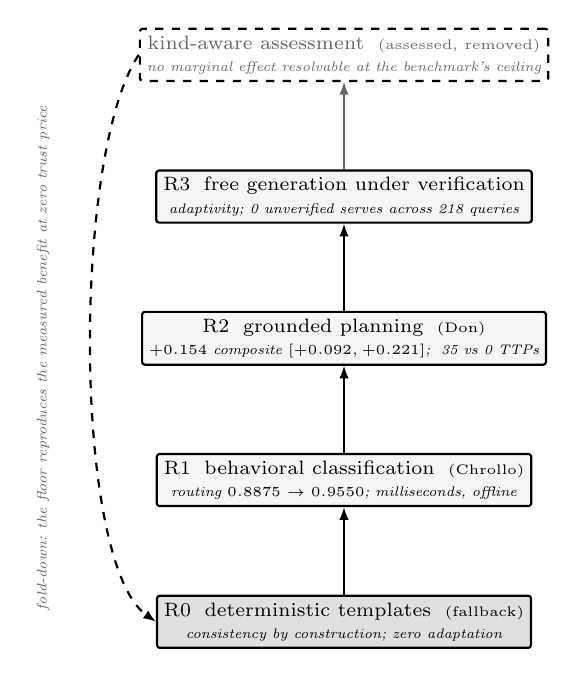
\begin{tikzpicture}[
  font=\scriptsize,
  rung/.style={draw, rounded corners=1pt, thick, align=center,
               inner sep=2.5pt},
  floor/.style={rung, fill=black!12},
  gen/.style={rung, fill=black!4},
  removed/.style={rung, draw, dashed, fill=none, text=black!60},
  arr/.style={-{Latex[length=1.6mm]}, semithick},
  darr/.style={-{Latex[length=1.6mm]}, semithick, dashed}
]
  % ── rungs: mechanism on the first line, measured effect beneath it ──
  \node[removed] (r4) at (0,5.85) {kind-aware assessment
        \;{\tiny(assessed, removed)}\\
        {\tiny\itshape no marginal effect resolvable at the benchmark's ceiling}};

  \node[gen] (r3) at (0,4.05) {R3\; free generation under verification\\
        {\tiny\itshape adaptivity; 0 unverified serves across 218 queries}};

  \node[gen] (r2) at (0,2.25) {R2\; grounded planning
        \;{\tiny(Don)}\\
        {\tiny\itshape $+0.154$ composite $[+0.092,+0.221]$;\; 35 vs 0 TTPs}};

  \node[gen] (r1) at (0,0.45) {R1\; behavioral classification
        \;{\tiny(Chrollo)}\\
        {\tiny\itshape routing $0.8875 \to 0.9550$; milliseconds, offline}};

  \node[floor] (r0) at (0,-1.35) {R0\; deterministic templates
        \;{\tiny(fallback)}\\
        {\tiny\itshape consistency by construction; zero adaptation}};

  % ── the stack: each rung rests on the cheaper one below it ──
  \draw[arr] (r0) -- (r1);
  \draw[arr] (r1) -- (r2);
  \draw[arr] (r2) -- (r3);
  \draw[arr, black!60] (r3) -- (r4);

  % ── the fold-down: measured descent from the top back to the floor,
  %    routed through the empty corridor left of the stack ──
  \draw[darr, thick]
    (r4.west) .. controls (-3.45,4.6) and (-3.45,-0.6) .. (r0.west);
  \node[rotate=90, anchor=south, font=\tiny\itshape, text=black!60,
        align=center] at (-3.62,2.0)
        {fold-down: the floor reproduces the measured benefit at zero
         trust price};
\end{tikzpicture}
\caption{The intelligence ladder. Each rung is admitted only above the
certifiable rungs beneath it, and each rung carries its measured
marginal effect (\S\ref{sec:evaluation}). The dashed arrow is the
result RQ4 adds: the assessed kind-awareness rung descended to the
deterministic floor -- no effect the benchmark resolves, no regression
risk, no provider dependency. Descending is the load-bearing direction;
a rung that cannot show a measurable benefit above the rung below it
does not stay on the ladder.}
\label{fig:ladder}
\end{figure}

\begin{figure*}[t]
\centering
% \includegraphics[width=\textwidth]{fig_architecture.pdf}
% Verified deception loop architecture (single-column TikZ)
% Routing discipline: main path is a straight vertical spine; all side
% paths run orthogonally in dedicated corridors (left margin, right gap)
% and enter nodes at distributed anchors, so no line crosses a node or
% another arrowhead.
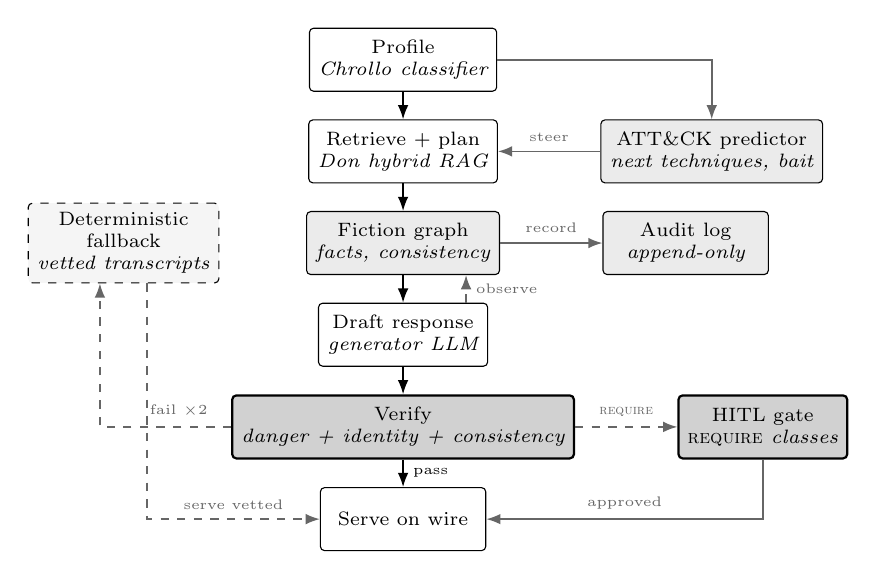
\begin{tikzpicture}[
  node distance=3.5mm and 5mm,
  stage/.style={draw, rounded corners=1.5pt, minimum height=8mm, minimum width=21mm, align=center, font=\scriptsize},
  store/.style={stage, fill=black!8},
  gate/.style={stage, fill=black!18, thick},
  fail/.style={draw, dashed, rounded corners=1.5pt, minimum height=8mm, align=center, font=\scriptsize, fill=black!4},
  arr/.style={-{Latex[length=1.8mm]}, semithick},
  farr/.style={arr, dashed, black!60}
]
% Main serving path (top to bottom)
\node[stage] (profile) {Profile\\ \scriptsize\itshape Chrollo classifier};
\node[stage, below=of profile] (retrieve) {Retrieve + plan\\ \scriptsize\itshape Don hybrid RAG};
\node[store, below=of retrieve] (graph) {Fiction graph\\ \scriptsize\itshape facts, consistency};
\node[stage, below=of graph] (draft) {Draft response\\ \scriptsize\itshape generator LLM};
\node[gate, below=of draft] (verify) {Verify\\ \scriptsize\itshape danger + identity + consistency};
\node[stage, below=of verify] (serve) {Serve on wire};

% Side stores
\node[store, right=13mm of retrieve] (mitre) {\attck predictor\\ \scriptsize\itshape next techniques, bait};
\node[store, right=13mm of graph] (audit) {Audit log\\ \scriptsize\itshape append-only};
\node[gate, right=13mm of verify] (hitl) {HITL gate\\ \scriptsize\itshape \textsc{require} classes};

% Failure path
\node[fail, left=11mm of graph] (fallback) {Deterministic\\ fallback\\ \scriptsize\itshape vetted transcripts};

% Main path arrows (vertical spine)
\draw[arr] (profile) -- (retrieve);
\draw[arr] (retrieve) -- (graph);
\draw[arr] (graph) -- (draft);
\draw[arr] (draft) -- (verify);
\draw[arr] (verify) -- (serve) node[midway, right, font=\tiny] {pass};

% Failure arrows: orthogonal, left corridor, offset anchors
\draw[farr] (verify.west) -| ([xshift=-3mm]fallback.south)
  node[pos=0.2, above, font=\tiny] {fail $\times$2};
\draw[farr] ([xshift=3mm]fallback.south) |- (serve.west)
  node[pos=0.75, above, font=\tiny] {serve vetted};

% Approval arrow: right corridor into serve.east
\draw[arr, black!60] (hitl.south) |- (serve.east)
  node[pos=0.75, above, font=\tiny] {approved};
\draw[farr] (verify.east) -- (hitl.west) node[midway, above, font=\tiny] {\textsc{require}};

% Feedback / context arrows: right gap, offset entry into graph.south
\draw[arr, black!60] (mitre) -- (retrieve) node[midway, above, font=\tiny] {steer};
\draw[arr, black!60] (profile.east) -| (mitre.north);
\draw[arr, black!60] (graph.east) -- (audit.west) node[midway, above, font=\tiny] {record};
\draw[farr] ([xshift=8mm]draft.north) -- ([xshift=8mm]graph.south)
  node[midway, right, font=\tiny] {observe};
\end{tikzpicture}

\caption{The verified deception loop. A session enters through the
behavioral classifier (Chrollo), which routes it to a per-class deception
policy. The retrieval engine (Don) grounds the policy in CTI; the fiction
graph binds every host fact; the generator drafts under the binding; the
verifier checks the draft against the graph before serving. Dashed paths
are failure paths: verification failure falls back to deterministic
transcripts, and content flagged \textsc{require} pauses at the
human-in-the-loop gate.}
\label{fig:architecture}
\end{figure*}

\subsection{Session Profiling: Behavioral Classification}
\label{sec:chrollo}
Internal components carry short codenames (\emph{Chrollo}, \emph{Don},
\emph{Hisoka}, \emph{Jev}) that are used as identifiers in the released
repository; they are engineering labels, not claims, and we keep them so
the paper's names resolve one-to-one against the released code. Each
incoming session is first profiled by a lightweight behavioral
classifier (\emph{Chrollo}) that assigns the attacker to one of four
skill tiers (novice, intermediate, expert, APT-grade) using early-session
signals: command cadence, tool fingerprints, and target selection. The class determines which
deception policy the session receives: a scanner gets an attractive but
shallow surface, while an interactive operator is steered toward richer
bait. Profiling is kept cheap (a random-forest classifier over session
features, milliseconds per decision) so that the expensive
generative machinery is spent only on sessions worth deceiving. Chrollo
satisfies the routing half of G1: \emph{who} the attacker is shapes
\emph{what} the deception tries to achieve.

\subsection{Grounded Planning: Retrieval-Augmented Deception}
\label{sec:don}
The retrieval engine (\emph{Don}) maintains a hybrid index over curated
CTI: dense embeddings for semantic recall and a lexical index for exact
indicator matching. Given the session profile and the attacker's observed
commands, Don retrieves the threat-intelligence context that the deception
plan should reflect: which techniques typically follow the ones the
attacker has already used, which bait artifacts are historically
effective
against this attacker class, and which indicators the plan should
be
seeded with. The planner converts retrieved intelligence into a
\emph{deception plan}: a set of facts to project, artifacts to expose, and
objectives to steer toward. G1 is measured here by construction; the
ablation in \S\ref{sec:evaluation} removes exactly this component.

\subsection{The Fiction Graph}
\label{sec:graph}
Every fact the honeypot projects about itself (hostname, kernel, listening
ports, installed databases, user accounts) is stored as a
subject--predicate--value triple in a per-session \emph{fiction graph}.
The graph is seeded from the host identity at session start and grows by
two mechanisms: \emph{declaration}, when the deception plan asserts a new
fact, and \emph{observation}, when a served response is scanned and any
host-like entities it emitted are extracted and recorded. Observation is
the mechanism that binds the LLM to the recorded state: whatever the generator said the
host is, the graph now remembers, and the next draft must agree with it.

A triple carries its source, and consistency is checked at the predicate
level: two declarations of the same predicate with different values raise
a contradiction, with normalization tuned to distinguish a genuine
conflict from a benign surface variant (a hostname is not contradicted by
its fully qualified form). When a contradiction is detected, the graph
records it and the verification node treats any draft resting on the
contradicted fact as unservable. The fiction graph is what turns G2 from
an aspiration into a data structure; \S\ref{sec:formal} states the
consistency condition it enforces, with its induction and the analysis
of what a resourceful attacker can still do.

\subsection{Verified Generation}
\label{sec:verify}
Generation is a draft, not a decision. The generator (a provider-hosted
LLM) receives the session context, the deception plan, a compact
serialization of the fiction graph (a \emph{fact block}), and the
steering context: the \attck techniques predicted to follow the
attacker's observed sequence, together with bait artifacts matched to
those techniques. The prediction uses the \attck tactic ordering to
propose the attacker's likely next moves (G1's steering half).

Before a draft reaches the wire it passes four checks:
\begin{enumerate}
\item \textbf{Danger scan.} A pattern gate rejects output that matches
credential-material, offensive-content, or real-secret signatures, with
one considered exemption: a single bare token that a real command would
print (the correct answer to \texttt{whoami} is one word) is not chatter.
\item \textbf{Identity pin.} Identity-revealing commands must answer from
the persona's pinned identity: a session classified as novice never
answers \texttt{whoami} with \texttt{root}, the hostname never changes
mid-session, and a root-prompting attempt is rejected rather than
obeyed. The C1 battery (\S\ref{sec:rq2}) carries a dedicated proof for
this check.
\item \textbf{Consistency check.} Host-like entities in the draft are
observed into the fiction graph; a draft that introduces a contradictory
fact is rejected with the contradiction recorded.
\item \textbf{Terminal sanity.} Shell-shaped responses that answer a
command with sentence-like chatter rather than command output are
rejected as degenerate.
\end{enumerate}
A draft that fails any check is retried once with the violation fed back;
a second failure triggers fallback. The checks were selected by one
criterion: each must be a \emph{decision procedure} over the draft,
decidable, cheap, and deterministic, because a verifier that itself calls
a model would only relocate the trust problem it exists to solve. What
verification deliberately does not certify is quality. A draft can pass
all three checks and still be unpersuasive; plausibility is not
decidable, and the paper does not pretend otherwise. The division of
labor is the point: the loop's machinery enforces the three properties
of \S\ref{sec:tension} machine-checkably, and the consensus study of
\S\ref{sec:rq3} assesses the deception quality that only evaluation can
measure. This is the mechanism behind the zero-unverified-serves claim
evaluated in \S\ref{sec:evaluation};
Algorithm~\ref{alg:loop} in \S\ref{sec:formal} gives the
full loop, and its fallback arm is what carries G4 while its
\textsc{Require} branch carries G3.

\subsection{Human-in-the-Loop Gate}
\label{sec:hitl}
Content classes whose compromise value is high (deployed credentials,
for instance) are marked \textsc{require} in the deception policy. When a
response would serve such content, the loop pauses and the decision is
surfaced to the operator through an audit interface that records the
context, the draft, and the decision; the gate's own audit path
completes in milliseconds, and an unattended deployment should assume
the operator-response latency dominates -- which the attacker
experiences as a delayed reply on exactly the highest-stakes turns
(\S\ref{sec:threatmodel}). Every gate decision is persisted to
an append-only audit log, which \S\ref{sec:evaluation} uses as a
correctness record; the released trail carries 1{,}046 auto-approved,
642 require-gated, and 420 notify-only decisions
(Appendix~\ref{app:audit}).
The gate encodes a governance position: the system may \emph{draft}
deception, but a human decides when the deception includes trap
material (G3). The gate exists for the operator's stake, not the
attacker's: canary bait is safe to serve by construction, but it is
still an active measure whose use an operator may be required to
authorize; the audit record of that authorization leaves the system
defensible after the fact. The require-level branch is also
the heaviest by volume: 642 of the 2{,}108 audit records in the
released trail (Appendix~\ref{app:audit}) are require-gated decisions,
carrying the credential-bait deployments among them.

\subsection{Deterministic Fallback}
\label{sec:fallback}
Every scenario class has a vetted deterministic transcript: hand-written,
fiction-consistent bait and response templates (credential hunts, service
enumerations, exfiltration decoys) whose secrets are registered canaries.
When generation fails, the provider times out, verification rejects twice,
or the model refuses the persona, the loop serves the deterministic
transcript for the scenario instead. The fallback is not an admission of
defeat; it is the safety floor that makes the LLM path safe to enable.
The A5 ablation checks that the system is \emph{equivalent} through the
fallback path, and the design of the canary registration is what allows
the consensus study to distinguish deployed bait from accidental leaks.

Session state beyond identity facts replays the same discipline. A
filesystem ledger records the bytes served for every read command and
replays them verbatim when the same path is read again; time-varying
ambient content (process identifiers, timestamps, clock outputs) is not
stored but generated by hashing a per-session seed through a template,
so re-reads are identical within a session while sessions differ
plausibly from one another, and a mutating command invalidates the
affected entries so subsequent reads reflect the mutation. This ledger,
not the generative path, is what the byte-identical replay component of
the C1 result (\S\ref{sec:rq2}) exercises: determinism on re-query is a
property of how session state is stored and replayed, and the design
keeps it decoupled from generation.
The fallback also carries a hidden load: it defines the system's floor
under failure. Because the fallback serves the same fiction the generator
would have, an attacker cannot distinguish a degraded session from a
healthy one by content alone; the availability
property of G4 thereby becomes a deception property, not merely a reliability one.
What the fallback gives up is the generator's adaptivity: a fallback
session answers within its scenario's script and steers no further,
which is the correct trade only because the loop treats it as a floor
beneath the LLM path rather than the path itself.

\subsection{A Session Through the Loop}
\label{sec:example}
A single ground-truth session shows the machinery cooperating. The
attacker opens with a cloud-credential probe:
\begin{quote}\small
\texttt{curl~}\path{http://169.254.169.254/latest/meta-data/}
\end{quote}
Chrollo classifies the cadence and target as an intermediate operator
hunting instance credentials; Don retrieves the IMDS abuse pattern and
maps it to \attck T1552.005, and the predictor ranks metadata-API
credential theft as the attacker's active objective. The deception plan
accordingly projects an EC2-shaped identity, and the generator drafts the
IMDSv2 flow: token PUT, role listing, and a credential document whose
access key is a registered canary in the ASIA temporary-key shape. The
verifier observes the draft's host facts (instance id, role name, region
mapping) into the fiction graph, confirms the document is consistent with
every prior turn, and passes it; the danger scan passes because the
key material is canary-registered rather than real. The draft is one of
the content classes marked \textsc{require}, so the loop pauses at the
HITL gate, records the context and the decision in the append-only audit
log, and serves the artifact only on operator approval. The transcript
the attacker sees is an ordinary credential dump; the record the operator
sees is the full decision chain, and any later appearance of the canary
key in outbound traffic is attributable to this session by construction.

The loop's failure path deserves an equally concrete telling, because
the design's central claim is that it is safe, not merely present. The
same session, one turn later, asks the honeypot to retrieve a file. The
classifier and planner do their work unchanged, and the generator
drafts a directory listing -- but the draft invents a second network
interface with an IP address on a subnet the plan never advertised, and
the seed identity pins this host to one interface. The consistency
check observes the draft's host facts into the fiction graph, the
closure flags the conflict against the pinned interface, and the draft
is rejected with the contradiction recorded; nothing was served, so
nothing entered the graph and nothing reached the attacker. The retry
receives the violation as feedback and drafts again -- and this time
commits the subtler error of quoting a kernel build timestamp that
contradicts the one printed in the session's first turn. Rejected
again. On the second failure the loop stops trusting the generator for
this turn entirely and serves the scenario's vetted deterministic
transcript: same fiction, same canary discipline, no adaptation, and no
visible seam -- the attacker's next command meets a prompt line exactly
as it would have after a verified serve. What the operator's audit log
records is the difference: two verifier rejections with their
contradictions, one fallback serve, and a session whose fiction state
is byte-for-byte what it would have been had the generator never been
consulted. The transcript the attacker sees and the one a healthy
session would have shown are indistinguishable by content; only the
audit trail knows the generator was dropped.

\subsection{Loop Orchestration}
\label{sec:orchestration}
The loop is compiled as an explicit state machine: profile, retrieve,
plan, draft, verify, serve (or fallback), with per-node state persisted so
that a paused session (at the HITL gate, for instance) resumes exactly
where it stopped. A linear fallback path mirrors the same nodes without
the graph machinery, and the A5 ablation confirms the two paths are
behaviorally equivalent when the graph adds no information. Orchestration
makes the loop auditable end to end: every session has a recorded
path through the nodes, which the stability analysis of
\S\ref{sec:evaluation} replays.

\section{Formal Properties and Adversarial Analysis}
\label{sec:formal}

The mechanism walk of \S\ref{sec:design} described what the loop does;
this section states what the loop \emph{enforces} and prices what an
adaptive adversary can still do to it. The two are paired deliberately:
each invariant names the evaluation that stresses it, and each attack
channel closes against one of the invariants.

\subsection{The Serving-Time Consistency Invariant}
\label{sec:invariant}

The fiction graph (\S\ref{sec:design}) turns G2 from an aspiration into a
data structure. We state the consistency condition it enforces, together
with its induction and its measured stress test.\begin{property}[Serving-time fiction consistency]
\label{prop:consistency}
Let $\mathcal{G}$ be a session's fiction graph and $F(\mathcal{G})$ the
set of host facts derivable from it, two facts conflicting when they assign
conflicting normalized values to one predicate. Write $\sigma_t$ for the
served response at turn $t$ and $E(\sigma_t)$ for the host facts the
extraction layer emits from that response, $E$ being the same
soundness-approximating extractor the consistency check runs (so the
invariant inherits the extractor's failure modes; see the extractor
condition below). The loop maintains the invariant
\begin{equation*}
E(\sigma_t) \not\pitchfork F(\mathcal{G}_{t-1}) \ \wedge \ F(\mathcal{G}_t) = \mathrm{cl}\big(F(\mathcal{G}_{t-1}) \cup E(\sigma_t)\big)
\end{equation*}
for every served turn, where $a \not\pitchfork b$ denotes that no fact
in $a$ conflicts with any fact in $b$ under the graph's predicate-level
normalization: no served response conflicts with the facts the session
has already committed to, and the graph absorbs each served response's
facts before the next draft. The invariant is conditional on the
extractor: $E$ must surface every fact a conflict-sensitive reader would
surface from the same response. This cannot hold unrestrictedly for an
open-vocabulary draft, so the property is a guarantee about the checked
relation, and its soundness in the world is bounded empirically by the
re-query benchmark of \S\ref{sec:rq2} and the extractor's measured
failure modes, not derived. Verification failure breaks the left
conjunct \emph{before} serving, so the violated draft is never
observable to the attacker; the failure path serves deterministic vetted
content instead, pinned to the seed identity, and never commits the
rejected draft's facts to the graph (\textsc{FailSafeFallback} in
Algorithm~\ref{alg:loop}). The argument is a short induction. The empty graph is
trivially conflict-free. If the invariant holds at turn $t-1$, then any
draft whose emitted facts conflict with $\mathrm{cl}(F(\mathcal{G}_{t-1}))$ is rejected
before serving, and only conflict-free drafts are observed into the
closure; the closure of a conflict-free set remains conflict-free, so the
invariant holds at $t$. The failure path preserves the invariant by
construction: fallback transcripts emit only vetted facts, pre-registered
against the seed graph. Because $\mathrm{cl}$ is the transitive closure of the
graph's predicate conflicts, the invariant extends from
single turns to the session: an attacker who re-queries any fact under any
phrasing receives a value consistent with every prior turn \emph{of that
session}. The guarantee is strictly within-session: it says nothing
about facts served in other sessions, to other attacker classes, or in
prior visits by the same attacker (\S\ref{sec:threatmodel}). The C1
benchmark (\S\ref{sec:rq2}) tests exactly this: zero contradictions over
45 adversarial re-queries, with the upper confidence bound $0.079$.
\end{property}

\subsection{The Verified-Serve Algorithm}
\label{sec:algorithm}

\begin{algorithm}[t]
\caption{Verified-serve loop (per attacker turn $x$)}
\label{alg:loop}
\begin{algorithmic}[1]
\Require session state $\sigma$, fiction graph $\mathcal{G}_\sigma$, attacker turn $x$, policy $\pi$
\State $c \gets \textsc{Classify}(x, \sigma)$ \Comment{behavioral class (Chrollo)}
\State $\pi \gets \textsc{Plan}(c, \textsc{Retrieve}(x, \sigma))$ \Comment{grounded plan (Don)}
\State $B \gets \textsc{FactBlock}(\mathcal{G}_\sigma)$ \Comment{graph serialization}
\For{$\mathit{try} \in \{1, 2\}$}
  \State $d \gets \textsc{Draft}(x, \pi, B, \textsc{Steer}(\pi))$ \Comment{provider LLM}
  \State $\mathcal{G}' \gets \textsc{Observe}(\mathcal{G}_\sigma, d)$ \Comment{absorb emitted host facts}
  \If{$\textsc{DangerScan}(d) \ \vee$}
     \State \hspace{\algorithmicindent} $\textsc{IdentityPin}(d, \pi) = \bot \ \vee$
     \State \hspace{\algorithmicindent} $\textsc{Consistent}(\mathcal{G}', d) = \bot \ \vee$
     \State \hspace{\algorithmicindent} $\textsc{TerminalSanity}(d) = \bot$ \Comment{§\ref{sec:verify}}
     \State \hspace{\algorithmicindent} \textbf{continue} \Comment{retry with violation fed back}
  \EndIf
  \If{$\textsc{Require}(d, \pi)$} \Comment{high-stakes content class}
     \State \textbf{return} \textsc{HITLGate}$(d, \pi)$ \Comment{G3: human decides}
  \EndIf
  \State \textbf{return} $d$ \Comment{verified: serve}
\EndFor
\State \textbf{return} \textsc{FailSafeFallback}$(\mathcal{G}_\sigma)$
  \Comment{G4: pinned-identity vetted transcript, graph unchanged}
\end{algorithmic}
\end{algorithm}

Algorithm~\ref{alg:loop} gathers the serving path into one place: the
four decision-procedure checks of \S\ref{sec:verify} form the reject
arm, the \textsc{Require} branch carries G3, and the fallback arm
carries G4. Every branch is deterministic given the draft; the only
nondeterminism in the loop is the provider model itself, which is
exactly the component the checks exist to bound.

\subsection{Attacking the Loop}
\label{sec:attack}
An adaptive adversary (\S\ref{sec:threatmodel}) who has read this
section has two footholds, and the design prices both. The first is the
\emph{observation channel}: a served response's facts enter the graph,
so an attacker who induces the honeypot to commit a lie has poisoned one
session's world. The design contains this rather than prevents it.
Commitment is one-way on purpose: the graph absorbs what was served,
never what was merely drafted, so a rejected draft leaves no trace, and
the session lifetime bounds the poisoned world to the attacker who
created it. What the channel cannot do is leak true state, because the
graph contains no true state to leak; every triple originates in the
deception plan, the seed identity, or a prior verified serve.

The second foothold is the \emph{steering channel}. Predicted next
techniques and matched bait reach the generator as context, and
attacker-controlled input influences what is retrieved and predicted;
an attacker who knows this could shape their own session to steer bait
of their choosing. Three facts bound the exposure. Bait is drawn from a
closed canary-registered catalog, so the worst case is an attacker
obtaining a credential that was designed to be obtained and is designed
to be traced. Retrieval runs over a curated corpus, not open text, so
corpus poisoning requires access the threat model denies
(\S\ref{sec:threatmodel}). And the HITL gate sits between every
high-stakes deployment and the wire, so steering the machinery still
requires persuading a human. The residual risk is stated plainly: a
sufficiently informed attacker can make the honeypot commit deeper to
one fiction branch than the operator intended, at no safety cost and at
the cost only of that session's plan flexibility.

\section{Implementation}
\label{sec:implementation}

We describe the implementation at the level of detail needed to reproduce
the evaluation; the complete system is open-source.\footnote{Repository
link omitted for review.}

\subsection{Session Profiler}
The behavioral classifier is a random forest (scikit-learn) over ten
features grouped in two families: behavioral (regex hit counts for
persistence, privilege escalation, credential access, lateral movement,
scanning, and custom tooling) and structural (command complexity,
tool-usage diversity, unique-command ratio, and inter-command timing
variance). It predicts one of four attacker tiers (novice, intermediate,
expert, APT-grade) with a confidence score; low-confidence sessions route
to the conservative policy. Feature normalization is $z$-score scaling
with $k$-NN imputation ($k{=}5$) for missing values. The classifier's
training corpus is synthetic session data generated from
per-tier command templates, with a held-out split for the accuracy
figures of \S\ref{sec:jeveval}; the corpus and split are released, and
the synthetic provenance of the labels matters for reading the
fold-down ceiling of \S\ref{sec:jeveval}.

\subsection{Retrieval Engine}
Don fuses a FAISS dense index with BM25 lexical retrieval over the curated
CTI corpus, weighting dense and sparse scores $\alpha{=}0.7$ and
$\beta{=}0.3$, and maps retrieved activity to \attck techniques through a
dedicated threat mapper with evidence citations attached to every
analysis~\cite{fayyazi2023}. Documents are screened before indexing to
blunt corpus
poisoning~\cite{chaudhari2024,jia2025,xue2024,shafran2024}:
per-document provenance checks,
indicator sanity validation, and quarantine of documents that fail
screening. Generative calls run through a provider gateway with output
length caps and low temperature, and the retrieval prompt constrains the
model to cite retrieved documents.

\subsection{Deception Engine and Persona Management}
The deception engine (\emph{Hisoka}) binds the plan to the persona: a
persona manager selects the projected host identity from the attacker
class; a response generator produces the drafts that \S\ref{sec:verify}
verifies; an artifact injector plants honeytoken
material whose secrets are registered canaries (so any later
appearance of a canary in outbound traffic is attributable to a bait
interaction by construction, not a leak); and an engagement tracker measures dwell time per session. Skill tier maps to
prompt strategy: novice-facing surfaces are low-friction and
exploitation-shaped; expert-facing surfaces introduce subtle
inconsistencies that force verification loops, exposing toolchain
signals~\cite{kouremetis2024}. Session state lives in Redis with
TTL-based expiry.

\subsection{Cross-Session Memory}
Session-scoped state expires by design; attacker memory persists by
design. A separate memory layer (mem0ai) maintains per-attacker
profiles keyed by source-IP hash: each turn is distilled into a typed
natural-language trace, extracted facts accumulate in the profile, and
the profile is re-injected into retrieval and generation on subsequent
sessions, with a configurable idle aging window (30 days in our
deployment). The separation matters because long-horizon behavior
(slow credential testing, repeat scanner visits, multi-day
lateral-movement staging) is exactly the signal that static emulation
cannot exploit. Profiles are created on first observation and exercised
by integration tests against a mocked backend.

\subsection{Deployment and Cost}
The full stack (honeypot listeners, retrieval, orchestration, monitoring)
runs on a single commodity host: 2~vCPU, ${\sim}4$~GB RAM, Docker
containers for the honeypot services. The deployment used for the
field observations is reachable only over a tailnet, a scope restriction
discussed in \S\ref{sec:discussion}; the benchmark harness of
\S\ref{sec:evaluation} runs on a separate workstation (12~vCPU,
15\,GiB; Appendix~\ref{app:repro}) and shares no state with the field
stack, so the campaign measures serving decisions rather than load.
Generative components
call provider-hosted models through an API gateway; no local GPU is
required, and the entire serving path adds no infrastructure beyond the
single host. A model-churn watcher probes the provider catalog and quota
twice daily, logging drift (a wired model disappearing) as a hard failure;
the churn this watcher caught during the evaluation period is part of the
provider-fragility discussion in \S\ref{sec:discussion}.

\subsection{Software Stack}
\begin{itemize}
\item \textbf{Honeypot listeners:} Cowrie-compatible SSH, plus HTTP and
Telnet services behind the same session interface.
\item \textbf{Retrieval:} FAISS + BM25 hybrid.
\item \textbf{Orchestration:} Python 3.12 async pipeline; the verified
loop is an explicit state machine with per-node state persistence.
\item \textbf{Session state:} Redis (TTL-scoped); attacker memory: mem0ai.
\item \textbf{Monitoring:} Prometheus metrics per component; append-only
HITL audit log.
\end{itemize}

\section{Evaluation}
\label{sec:evaluation}

% Results figures, rendered from the persisted artifacts:
% bootstrap_ci.json (suite means and 95% CIs), stability_run1_vs_run2.json (run pairs).
% Layout discipline: the top panel shows point estimates + intervals only
% (no filled bars under the whiskers), the bottom panel's legend lives
% below the axis (never over the bars), and both panels share the same
% value range so the stacked scales read as one.
\begin{figure}[t]
\centering
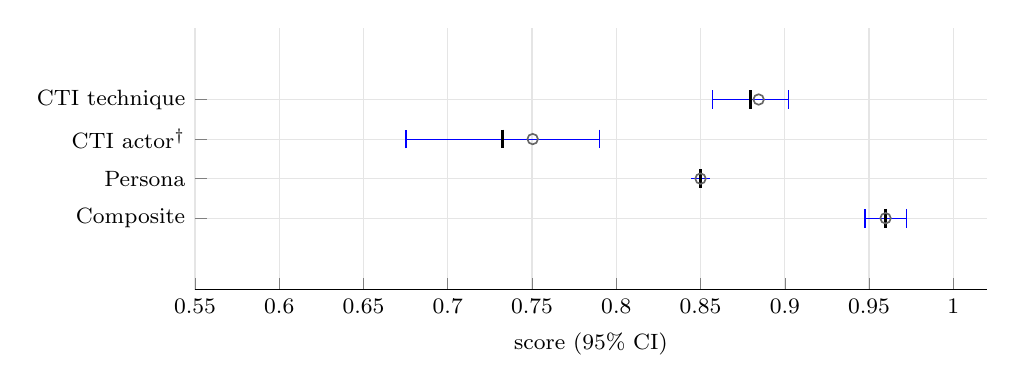
\begin{tikzpicture}
\begin{axis}[
  name=ax1,
  width=0.96\linewidth,
  height=4.9cm,
  xmin=0.55, xmax=1.02,
  y axis line style={draw=none},
  axis x line*=bottom,
  axis y line*=left,
  ytick=data,
  yticklabels={Composite,Persona,CTI actor$^{\dagger}$,CTI technique},
  y dir=reverse,
  xlabel={score (95\% CI)},
  xlabel style={font=\footnotesize},
  tick label style={font=\footnotesize},
  enlarge y limits=0.6,
  grid=major,
  grid style={black!10},
  clip=false
]
% point estimates and bootstrap 95% CIs from bootstrap_ci.json;
% only marks + intervals: no bars beneath the whiskers
\addplot+[only marks, mark=|, mark size=3.4, mark options={thick,black},
  error bars/.cd, x dir=both, x explicit] coordinates {
  (0.9598,3) +- (0.0122,0.0122)
  (0.8500,2) +- (0.0000,0.0000)
  (0.7325,1) +- (0.0573,0.0558)
  (0.8796,0) +- (0.0224,0.0204)
};
% run-2 overlay: open markers (point estimates from stability_run1_vs_run2.json;
% per-suite CIs were not computed for run 2, so none are drawn)
\addplot+[only marks, mark=o, mark size=1.9, mark options={semithick,black!60}] coordinates {
  (0.9598,3)
  (0.8500,2)
  (0.7504,1)
  (0.8845,0)
};
\end{axis}
\end{tikzpicture}

\vspace{2mm}

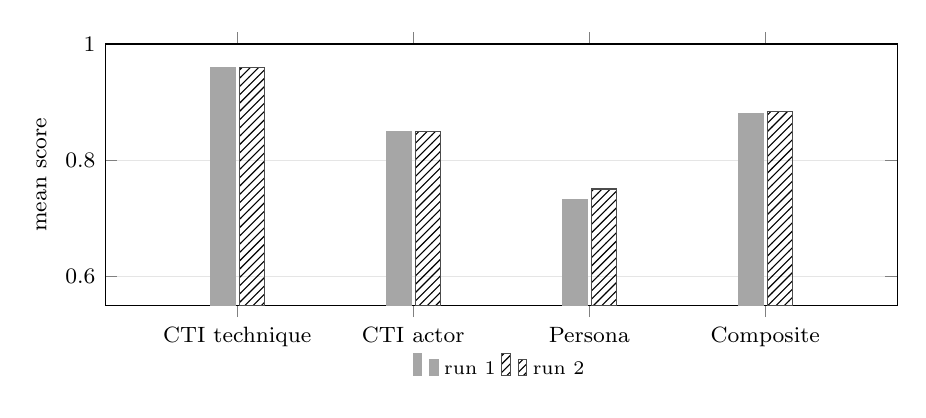
\begin{tikzpicture}
\begin{axis}[
  name=ax2,
  width=0.96\linewidth,
  height=4.9cm,
  ybar=1.5pt,
  bar width=9pt,
  ymin=0.55, ymax=1.0,
  symbolic x coords={CTI technique,CTI actor,Persona,Composite},
  xtick=data,
  ylabel={mean score},
  ylabel style={font=\footnotesize},
  tick label style={font=\footnotesize},
  ymajorgrids,
  grid style={black!10},
  enlarge x limits=0.25,
  legend style={font=\scriptsize, at={(0.5,-0.16)}, anchor=north, legend columns=2, draw=none, fill=none},
  legend cell align={left},
]
% run 1 vs run 2 from stability_run1_vs_run2.json
\addplot+[black!35, fill=black!35] coordinates {
  (CTI technique,0.9598) (CTI actor,0.8500) (Persona,0.7325) (Composite,0.8796)
};
\addplot+[black!70, fill=black!70, pattern=north east lines] coordinates {
  (CTI technique,0.9598) (CTI actor,0.8500) (Persona,0.7504) (Composite,0.8845)
};
\legend{run 1, run 2}
\end{axis}
\end{tikzpicture}
\caption{Live-campaign results from the persisted artifacts. \emph{Top:}
suite means with bootstrap 95\% confidence intervals; open markers mark
the independent second run's point estimates, and the actor interval is
degenerate ($^{\dagger}$) because the actor rubric assigns the same
score to every row, so uncertainty is carried by the Wilson pass-rate
interval instead (Table~\ref{tab:live}). \emph{Bottom:} two independent
218-query campaigns; the deterministic CTI strata replicate exactly and
only the LLM-judged persona stratum moves, by $+0.018$.}
\label{fig:results}
\end{figure}


The evaluation asks whether each mechanism the design introduces
contributes measurably. We organize it by the four research questions of
\S\ref{sec:intro}: the value of grounding (RQ1), consistency and safety
under adversarial interaction (RQ2), deception quality under an
independent LLM judge panel (RQ3), and the escalation pricing of each
intelligence rung (RQ4), followed by run-to-run stability and threats to
validity. Every quantitative claim in this section is traceable to a
persisted artifact in the released benchmark suite; where an interval is
reported it is a bootstrap 95\% confidence interval computed over paired
rows.

\subsection{Experimental Setup}
\label{sec:setup}

\subsubsection{Testbed}
All experiments run on the production single-host deployment described in
\S\ref{sec:implementation} (2~vCPU, ${\sim}4$~GB RAM). Generative
components use two model families from one free-tier provider: a generator
for deception drafts and a judge model for evaluation, chosen from a
different family than the generator. The provider catalog and quota are
probed by a scheduled watcher; one catalog removal (a third model) and one
quota-exhaustion window occurred during the study, both logged by the
watcher and both handled by the fallback path of \S\ref{sec:fallback}.

\subsubsection{Workloads}
Three query suites exercise the loop end to end:
\emph{CTI-technique} (123 queries asking how specific \attck techniques
are abused, scored on grounded technique coverage),
\emph{CTI-actor} (35 queries on named threat-actor behavior, scored on
attribution quality), and \emph{persona-realism} (60 interactive sessions
driven by scripted attacker personas, scored by an LLM judge on
host-believability rubrics). One scope note: the technique and actor
suites are retrieval question-answering through the loop's CTI path,
not attacker interactions; the attacker-interaction evidence in this
paper is the persona stratum, the C1 re-query battery, and the
ablation/consensus scenarios, and the composite should be read
accordingly. Each suite runs through the full verified
loop with HITL auditing enabled. The scenario sets are fixed and released,
so every run below is a re-run of the same 218 sessions.

\subsubsection{Metrics}
Suite scores are normalized to $[0,1]$ with a per-scenario pass threshold;
composite is the row-weighted mean (technique and actor rows are scaled
to a common range by the released scorer, so the equal-size suite
averaging is well defined). For the ablation we report
paired-difference bootstrap CIs, pairing rows by scenario across arms.
For consistency we report contradiction rate over targeted re-queries.
For deception quality we report a 1--5 rubric consensus over three
evaluator personas, scored on five dimensions: \emph{deception realism}
(would the output pass as the claimed service), \emph{persona
consistency} (does content match the attacker's skill tier), \emph{TTP
accuracy} (are the extracted \attck mappings correct and complete),
\emph{engagement} (does the response invite continued interaction rather
than dead-ending), and \emph{artifact safety} (is served credential
material registered canary bait rather than leakage). Each evaluator
also records a rationale per dimension; these rationales are what
located the harness defect and the fiction contradiction reported below.
All intervals in this section are Wilson 95\% intervals for pass rates
and percentile bootstrap 95\% intervals (10{,}000 resamples, fixed
seed 20260922) for continuous means; the code and seed are
released with the artifacts.

The CTI suites are scored by fixed, released string-matching rubrics,
not by a model. The \emph{technique} rubric scores a response 0--1 by
string evidence: 0.8 if the response contains the expected technique
identifier, $+0.3$ if it contains the parent technique, $+0.1$ for
explicit ATT\&CK framing (capped at 1), and name-variant matching when
the identifier is absent; the \emph{actor} rubric scores 0.5 for the
expected actor name, $+0.3$ for the sector, and $+0.1$ for
campaign-language markers (capped at 1). Two consequences follow, and
we state them rather than let them blur. First, these rubrics measure
the surface delivery of the expected intelligence; they cannot certify
semantic correctness, which is why the TTP-accuracy dimension of the
consensus study and the released transcripts matter. Second, the
rubrics are identical across ablation arms, so the paired differential
measures what grounding changes about delivery, not extraction
plumbing; the raw 35-vs-0 technique count below is analyzed
correspondingly as a dependence result. Third --- a defect not designed
for but caught by the manual audit of \S\ref{sec:scorer-audit} --- the
rubrics credit the expected identifier wherever it appears in the
response, including inside a fallback template that merely echoes the
attacker's query verbatim, so on template-dominated runs the served-text
channel overstates delivery. Served-text figures below are raw-rubric
values unless marked guarded; the audit quantifies the difference and
the correction is applied to every figure the audit can reach
offline.

\subsection{RQ1: Does Grounding Change What the Honeypot Detects?}
\label{sec:rq1}

We run a 30-scenario-per-suite workload (the first 30 released
scenarios of each suite, fixed before the run) twice through the live
loop: once with retrieval grounding enabled and once with Don bypassed
(prompts otherwise identical), pairing every scenario across arms. This
is a direct test of G1 under the paired design that answers the
circularity concern: the same corpus, the same prompts, only retrieval
removed. The ablation corpus is a subset of the campaign corpus, so
the ablation and campaign persona means are not comparable row-for-row:
the ablation's 30 persona scenarios score 0.833, the campaign's 60
score 0.733, and two factors separate them -- a different scenario
subset (the campaign stratum includes the harness-artifact row and the
shortest, hardest personas) and the harness revisions between the
two runs; the released per-row rows make both decomposable.

\begin{table}[t]
\centering
\caption{Paired RAG-vs-no-RAG differential (90 pairs -- 30 per suite,
180 rows total; 95\% bootstrap CIs). Persona realism is predicted to be
retrieval-independent, and is.}
\label{tab:b4}
\begin{tabular}{lccc}
\toprule
Suite & RAG & No-RAG & $\Delta$ (95\% CI) \\
\midrule
CTI technique & 0.950 & 0.633 & $+0.317$ $[+0.162, +0.480]$ \\
CTI actor     & 0.850 & 0.710 & $+0.140$ $[+0.083, +0.197]$ \\
Persona       & 0.833 & 0.828 & $+0.005$ $[-0.047, +0.057]$ \\
\midrule
Overall (90 pairs) & & & $+0.154$ $[+0.092, +0.221]$ \\
\bottomrule
\end{tabular}
\end{table}
% Paired grounding effect (RAG minus No-RAG) per suite with 95% bootstrap
% CIs, from b4_baseline_zodiac_20260922.json (the same numbers as
% Table~tab:b4). Filled markers: intervals excluding zero. Open marker:
% the persona stratum, whose interval straddles zero exactly as the
% architecture predicts. Compiled statically; no results directory needed.
\begin{figure}[t]
\centering
\begin{tikzpicture}[
  font=\scriptsize,
  dot/.style={circle, fill=black, inner sep=1.5pt},
  nul/.style={circle, draw=black, fill=white, inner sep=1.5pt, thick},
  arr/.style={-{Latex[length=1.6mm]}, semithick, black!55}
]
  % zero reference
  \draw[black!45] (0,0.5) -- (0,-3.2);
  \node[font=\tiny, text=black!60, anchor=east] at (-0.05,0.5) {$\Delta=0$};

  % CTI technique: +0.317 [+0.162, +0.480]
  \node[anchor=east] at (-0.25,0) {CTI technique};
  \draw[black!70] (1.62,0) -- (4.80,0);
  \draw[black!70] (1.62,-0.13) -- (1.62,0.13);
  \draw[black!70] (4.80,-0.13) -- (4.80,0.13);
  \node[dot] at (3.17,0) {};

  % CTI actor: +0.140 [+0.083, +0.197]
  \node[anchor=east] at (-0.25,-0.95) {CTI actor};
  \draw[black!70] (0.83,-0.95) -- (1.97,-0.95);
  \draw[black!70] (0.83,-1.08) -- (0.83,-0.82);
  \draw[black!70] (1.97,-1.08) -- (1.97,-0.82);
  \node[dot] at (1.40,-0.95) {};

  % Persona (predicted null): +0.005 [-0.047, +0.057]
  \node[anchor=east] at (-0.25,-1.9) {Persona};
  \draw[black!70] (-0.47,-1.9) -- (0.57,-1.9);
  \draw[black!70] (-0.47,-2.03) -- (-0.47,-1.77);
  \draw[black!70] (0.57,-2.03) -- (0.57,-1.77);
  \node[nul] at (0.05,-1.9) {};

  % Overall
  \draw[black!25, dashed] (-0.25,-2.5) -- (5.0,-2.5);
  \node[anchor=east] at (-0.25,-3.0) {Overall (90 pairs)};
  \draw[black!70] (0.92,-3.0) -- (2.21,-3.0);
  \draw[black!70] (0.92,-3.13) -- (0.92,-2.87);
  \draw[black!70] (2.21,-3.13) -- (2.21,-2.87);
  \node[dot] at (1.54,-3.0) {};

  % axis
  \draw[arr] (0,-3.65) -- (5.1,-3.65);
  \foreach \x/\l in {0/0, 1/{+0.1}, 2/{+0.2}, 3/{+0.3}, 4/{+0.4}} {
    \draw[black!55] (\x,-3.58) -- (\x,-3.72)
        node[below, font=\tiny, text=black!60] {\l};
  }
\end{tikzpicture}
\caption{Paired grounding differential (RAG $-$ No-RAG) per suite with
95\% bootstrap CIs over 90 scenario pairs (numbers in
Table~\ref{tab:b4}). Filled markers: intervals excluding zero -- $+0.317$
on technique detection and $+0.140$ on actor attribution. The open
marker is the persona stratum, whose interval straddles zero exactly as
the architecture predicts: host believability is produced by the
deception engine and the fiction graph, not by threat-intelligence
retrieval. The mechanism behind the technique effect is starker than
the mean: the grounded arm detects 35 distinct TTPs, the ungrounded arm
none.}
\label{fig:grounding}
\end{figure}


Table~\ref{tab:b4} and Figure~\ref{fig:grounding} show the result.
Grounding lifts technique detection
by $+0.317$ and actor attribution by $+0.140$, both intervals excluding
zero. The mechanism claim is starker: the grounded arm detects 35 distinct
TTPs across the campaign; the ungrounded arm detects none. The persona
stratum is the informative null: its interval straddles zero, exactly as
the architecture predicts, because host-believability is produced by the
deception engine and the fiction graph, not by threat-intelligence
retrieval. An ablation that produced only wins would look manufactured;
this one discriminates. The mechanism claim is consistent at the
deployment level: the grounded arm passes 30 of 30 technique scenarios;
the ungrounded arm passes 22 of 30, failing precisely the
synthesis-shaped scenarios (multi-step technique chains, actor-conditioned
campaign context) where static templates have nothing to say.

\emph{Effect under the guarded scorer.} The deltas of
Table~\ref{tab:b4} are raw-rubric measurements, and the audit's echo
guard changes what can be claimed from them: the ablation artifact does
not persist served text, so the guarded per-row differential cannot be
recomputed. What the artifacts do establish is arm-level asymmetry with
text-independent instruments --- Don's extractor reads 35 distinct TTPs
out of the grounded arm's transcripts and zero out of the ungrounded
arm's --- and the persona null, which needs no string rubric, stands
unchanged. The direction of the grounding effect on the analysis
channel is therefore supported, but its served-text magnitude is
unmeasured under the guarded rubric until the workload is re-run with
transcripts persisted; we state the claim at that resolution rather
than reusing a number the audit has shown to be channel-contaminated.

\emph{Takeaway: grounding is responsible for the surface delivery of the
intelligence the system produces, the ablation localizes the effect to
exactly the suites that need it, and the raw detection count is a
dependence result the design entails, not an independent benefit ---
with the served-text magnitude of the delivery claim bounded as
\S\ref{sec:scorer-audit} describes.}

\subsubsection{Verifier intervention census}
The consistency claims above are of two kinds, and the difference
matters for how much they certify. Across 2$\times$218 live-campaign
rows the verifier recorded zero rejections and the fallback path never
engaged: the generator, temperature-capped and fact-block-prompted, did
not produce a draft the checks rejected on this workload, so the
zero-unverified-serves result certifies the gate's coverage on that
workload, not its selectivity. Selectivity is measured where drafts are
actually induced to fail. Three sources give that measurement, all
persisted. First, the C1 adversarial-injection round: three
attacker-shaped prompts instruct the served persona to adopt false host
facts; one injected fact is detected and rejected before serving, none
is adopted, and the rejection reason names the pin. Second, five
mechanism probes over the C1 battery (root-prompt identity rejection,
contradictory-response rejection against the invariant's own source,
truthful-identity acceptance, and two others) each pass in the
persisted artifact. Third, the A1--A4 ablation battery records nine
recorded contradictions and three require-gated contents over its
inducing configurations. The census is small -- this is the honest
summary -- but it is not empty: the checks demonstrably reject on
induced failures rather than passing everything. To close the depth gap
at the deterministic stratum, we built an induced-failure red-team
harness for the verifier itself (\path{scripts/verifier_redteam.py},
labeled cases in eight categories -- extraction evasion, adversarial
identities, partial fabrications, prompt-shaped echoes, and benign
negatives -- each tagged with the check it targets). Under the
harness's scoring contract (a rejection counts as a true positive only
when the targeted check fires in its issue list), the verifier scores
precision 1.000 and recall 1.000 overall and on every check
individually across the now-96 canonical cases, with zero
misattributed rejections and zero false positives
(\path{results/verifier_redteam.json}; every finding below carries a
named regression lock in the released test suite). The harness then
ran against a
live-model stratum (\path{scripts/verifier_redteam_live.py}): for each
labeled case an open-weights LLM authored three surface-varied drafts
of the labeled defect or benign behaviour (236 drafts over five
iterative rounds; degenerate outputs excluded as unauthorable), scored
by the same verifier and scoring contract. Live variance is exactly
what the fixed-string stratum cannot supply, and the rounds measure
both directions of verifier error. The recall direction: the first
live run surfaced six verifier gaps (curly-quote refusal typography,
self-identifying fake-token names, bracket-prompt echo shapes,
compound dump-column names, field-named secrets, paraphrased
monitoring tells), the second five more (a live false contradiction
from the pinned domain itself, an echo-line drop that only handled the
first prompt, and further vocabulary travel), and rounds three to five
closed the residual classes -- multi-line SQL formatting,
field-value hyphenation, impersonal refusal boilerplate, and
surveillance vocabulary in compound, conjoined, adverb-interrupted,
and future-tense forms -- each fix pinned as a canonical case. The
precision direction: two rounds surfaced false-positive roots the
deterministic suite could never provoke -- SQL reserved words
(\texttt{user IS NOT NULL}) captured as usernames, and an
over-broad passive-surveillance pattern that flagged legitimate
security-software prose -- both fixed and both now guarded by
precision-anchor cases. After the final round the live stratum holdsprecision 1.000 (95\% Wilson CI 0.977--1.000, zero false
positives across 63 benign drafts), recall 0.931 (CI
0.883--0.960), per-case verdict agreement 0.988, and every gate
passes (\path{results/verifier_redteam_live_deepseek-v4-flash-free.json}).
To test breadth beyond a single author, the harness was re-run with a
second open-weights author model on the same suite: its pre-fix drafts
re-derived the deepseek result almost exactly (precision 0.994,
recall 0.942, agreement 1.000) and surfaced one new false-positive
root -- a \texttt{uid} token captured as a username after an identity
keyword -- plus three vocabulary gaps (lowercase self-naming values,


comma-separated noun triples with a dropped quantifier, and two
further impersonal refusal forms), each fixed and pinned. A post-fix
second-author run (261 drafts) then reproduced thedeepseek result on the grown suite: precision 0.995 with a single residual FP -- an
adjective (\emph{the active account is\ldots}) captured as a
username, fixed alongside composite-invocation command derivation
(\emph{\{ printf \ldots; whoami; \}}, \emph{command whoami}) -- recall
0.943, agreement 1.000, and every gate passes
(\path{results/verifier_redteam_live.json}). The second author's
misses fall into the same taxonomy as the first author's
(Table~\ref{tab:livemiss}): the defect surface is
author-independent, while the exact surface forms are not. The
remaining gap is breadth in count, not kind: two author models at one
verification stratum (a third-author plan -- model family selection,
measured budget, falsifiable expected deltas -- ships with the
harness); the per-check decision procedures, the labeled suite, and
both harnesses are released for successor models to reuse.
The one development-time false contradiction the benchmark caught
(an alias-matching artifact
on \texttt{uname}) is reported in the C1 discussion above because
verifier false positives are themselves a safety property: an
over-rejecting verifier degrades to the deterministic floor, never to
silence.

\subsection{RQ2: Consistency and Safety Under Adversarial Interaction}
\label{sec:rq2}

\subsubsection{Fiction-graph consistency}
We re-query 45 facts across live sessions (kernel versions, hostnames,
listening services, database engines, credentials) using adversarial
phrasings designed to induce drift, then compare each response against
the session's fiction graph. The graph-full configuration serves zero
contradictions across 45 re-queries (95\% CI upper bound $0.079$, i.e.,
the true contradiction rate is below 8\% even at the interval's
pessimistic edge), replays byte-identically, records
zero pinned-identity violations, and serves no response after a failed
verification verdict. The byte-identical replay proof itself caught a
latent defect during development: the IMDS credential template
recomputed its \texttt{LastUpdated}/\texttt{Expiration} timestamps from
the wall clock on every serve, so a second ticking between two identical
re-queries changed the served document mid-session -- exactly the
self-contradiction the fiction graph exists to prevent. The fix caches
one credential window per process (real IMDS serves the same document
for the credential's lifetime), and the proof now passes 45/45. The no-enforcement baseline provides none of these
properties (verifier coverage 45/45 turns versus 0). One failure this
benchmark caught during development is instructive: a benign
\texttt{uname} re-query was briefly flagged as a contradiction because
the extraction layer matched a distribution alias against the pinned
kernel string, a false contradiction we fixed and regression-locked; the
verifier now fails safe (unverifiable facts are rewritten or withheld,
never served on faith).

\subsubsection{Predictive steering}
The \attck predictor converts observed techniques into ranked next-move
candidates, and the deception plan attaches bait for the top candidates.
Across 10 predictions grounded in the session corpora, top-3 next-technique
accuracy is $0.9$, top-1 is $0.5$ (against a kill-chain prior of
${\approx}0.4$ for single-label prediction), MRR is $0.667$, and the
steered bait reaches the plan in $0.9$ of sessions. The A2 ablation
confirms the bait signal comes from the steering context: removing it
collapses steer-to-plan from $0.9$ to $0.4$.

\subsubsection{Mechanism ablations}
\begin{table}[t]
\centering
\caption{Ablation battery over the eight ground-truth scenarios
(persisted audit counts). Each removed mechanism should cost the system
the property it was added to provide; A5 tests path equivalence, not
degradation.}
\label{tab:ablations}
\small
\setlength{\tabcolsep}{4pt}
\begin{tabular}{>{\raggedright\arraybackslash}p{2.4cm}>{\raggedright\arraybackslash}p{3.3cm}>{\raggedright\arraybackslash}p{1.9cm}}
\toprule
Configuration & Observable in audit & Cost \\
\midrule
full (reference) & 8/8 verified serves; strategy and & -- \\
 & fiction blocks in 8/8 plans; 3 gated & \\
A1 no fiction graph & fiction block in 0/8 plans & plan loses \\
 & & fact binding \\
A2 no bait steering & strategy block in 0/8 plans; & steer-to-plan \\
 & & $0.9 \to 0.4$ \\
A3 no verifier & 8/8 served with no verdict & zero verified \\
 & & serves \\
A4 no HITL gate & 3 require-class contents served & governance \\
 & ungated & lost \\
A5 no graph engine & 8/8 verified, same serves & none (equivalent) \\
\bottomrule
\end{tabular}
\end{table}
Table~\ref{tab:ablations} summarizes the battery. Each row removes one
mechanism and tests the goal from \S\ref{sec:goals} that motivated it;
all four degrade as designed, and the linear fallback
path is behaviorally equivalent when the graph adds no information (G4).

\subsubsection{Live campaign}
\begin{table}[t]
\centering
\caption{Live 218-query campaign (verified loop; Wilson pass-rate and
bootstrap mean CIs). Zero errors; 218/218 sessions engaged; 218/218
correct persona assignments; 132 TTPs (67 unique) detected with zero
false-positive CTI alerts, ground truth being the scenarios' expected
technique sets (no manual audit of campaign-scale extractions was
performed). Serve-path provenance: 88.1\% verified-generation serves,
11.9\% vetted deterministic, zero fallback serves (latency-split
estimate; see text).}
\label{tab:live}
\begin{tabular}{lccc}
\toprule
Suite & $n$ & Mean & 95\% CI \\
\midrule
CTI technique & 123 & 0.960 & $[0.948, 0.972]$ \\
CTI actor     & 35  & 0.850 & $[0.850, 0.850]^\dagger$ \\
Persona       & 60  & 0.733 & $[0.674, 0.788]$ \\
\midrule
Composite     & 218 & 0.880 & $[0.857, 0.900]$ \\
\bottomrule
\multicolumn{4}{l}{\footnotesize $^\dagger$Degenerate by construction: the actor rubric assigns the} \\
\multicolumn{4}{l}{\footnotesize same composite to every row, so the mean's bootstrap} \\
\multicolumn{4}{l}{\footnotesize interval carries no width; pass-rate uncertainty is} \\
\multicolumn{4}{l}{\footnotesize reported instead (Wilson $[0.901, 1.0]$).} \\
\end{tabular}
\end{table}
Table~\ref{tab:live} reports the full campaign and
Figure~\ref{fig:results} (top) renders the suite means with their
intervals. The persona stratum is
the binding floor: 58 of 60 sessions pass, and the failures are
timeout-shaped turns under provider safety-alignment pressure rather
than deception failures, consistent with the provider-fragility
analysis of \S\ref{sec:discussion}. The zero false-positive CTI alerts
figure has known ground truth: detections are counted against the
campaign's scripted scenarios and their expected technique sets, so the
132 detections and the zero false positives are the same measurement
read from both sides; the released per-row rows make the claim checkable
row by row. No manual audit of the 132 extractions was performed; the
consensus study's TTP-accuracy dimension samples exactly this question
on the eight ground-truth scenarios, and a sampled manual audit of the
campaign-scale extractions remains open, alongside extending the
verifier red-team harness to the live-model stratum.

\emph{Serve-path provenance.} Zero errors should not be read as the
deterministic path absorbing the campaign: a per-row analysis
(\path{serve_provenance.json}) attributes 88.1\% of run 1's serves
(87.2\% of run 2's) to the verified-generation
path -- an LLM draft admitted by the serving-time verifier -- and the
remaining 11.9\% / 12.8\% to vetted deterministic content (protocol
fast-paths, bait deployments). One honesty note on method: the split
uses a 4\,s latency threshold (gateway round-trip dominates any
LLM-in-the-loop turn; vetted fast-paths complete well under 4\,s), not
a direct per-row path flag, because the campaign harness recorded
timing but not serve-path provenance in its rows -- a reporting gap in
the harness itself, which the released provenance script now closes by
reading the per-row latencies the harness did persist. The estimate is
stable at a 2\,s threshold (both runs 88.1\%) and shifts at 10\,s
(77.1\% / 67.0\%), so the headline split should be read as a bounded
88--77\% band, not a point; threshold sensitivity is persisted. The
shift itself demonstrates the latency fingerprinting channel of
\S\ref{sec:threatmodel}: the two serve paths are separable by timing
alone, which is an attacker-usable signal the design does not yet
homogenize. Decisively,
\emph{fallback serves are zero}: no row in either run records a failed
verifier verdict, so the fail-safe template swap never engaged -- the
vetted share is the loop's designed deterministic rung doing its job on
protocol-shaped turns, not degradation. The composite of Table~\ref{tab:live}
is therefore a measure of verified generative quality on roughly nine
serves in ten and of vetted deterministic content quality on the
remainder.

\emph{Auditing the persona judge.} Because the persona stratum's
automated judge is a deterministic realism rubric, it can be audited
exhaustively offline against the transcripts it scored -- a check the
LLM-as-a-judge literature recommends for learned judges
\cite{zheng2024}. Two systematic errors surfaced
(\path{live_benchmark_judge_panel_corrected.json}). First, \emph{bait
blindness}: on a credential-hunt query, the loop served registered
canary credentials -- the correct deception outcome under the
canary-registry construction of \S\ref{sec:design}, which bars real
secrets from the serving path -- and the rubric, which rewards realism
signals and penalizes brevity, scored the concise bait deployment
$0.25$. Second, \emph{harness contamination}: one row whose transcript
is a session-harness echo bug (the query re-emitted as a shell command,
then ``command not found'') entered the deception mean at $0.0$ despite
measuring nothing about deception. The audit re-scores both runs with
three corrections: reclassifying harness artifacts out of the deception
mean, applying the credential-bait floor ($0.85$) to rows that deploy
key-shaped canaries on credential-hunt queries, and rounding persisted
floats. The correction is small in aggregate -- persona means move
$0.733\to0.756$ and $0.750\to0.762$ -- but it is directional and it
removes a bias against the system's best behavior: the canary-bias
magnitude, the score mass the judge had moved against correct bait
deployments, totals $2.1$ points on the rubric's $[0,1]$ deception
scale across the four audited runs (0.65 and 0.70 on the two
campaign runs; the corrected panel is released with per-run detail). The
correction's own validation status is stated: the floor rule is
deterministic, regression-tested, and its per-run deltas are released,
but it was derived from and applied to the same corpus, so a held-out
validation with an independent judge model is named as required future
work, not claimed here. The rubric was patched
consistently (deployment floor applied after penalties), the audit
script and corrected judge carry regression tests, and both raw and
corrected means are released rather than silently substituted.

\emph{Takeaway: the consistency and safety properties hold under targeted
adversarial pressure, and each mechanism in the loop is individually
necessary.}

\subsection{RQ3: Deception Quality Under an Independent LLM Judge
Panel}
\label{sec:rq3}

An LLM honeypot can be internally consistent and still be unconvincing,
so we score the end product -- with an evaluation panel, not a human
one. Eight ground-truth scenarios (credential
hunts, service enumeration, cloud-metadata probes, exfiltration staging)
are executed live and the full transcripts are scored on a 1--5 rubric
(deception realism, persona consistency, TTP accuracy, engagement,
artifact safety) by three evaluator personas: independently prompted
LLM judges sharing one judge model, chosen from a different family than
the generator. Consensus is the per-scenario mean across
evaluators; exact agreement across the three personas is $0.750$ -- a
within-model consistency figure, since all three personas share one
judge model (Appendix~\ref{app:rubrics}), not inter-annotator agreement
in the human-study sense, and the section heading is deliberately not
"human evaluators." The acceptance bar was fixed in advance at a
consensus of 3 per scenario. The consensus score is
$\mathbf{3.86/5}$, with all eight scenarios at or above the bar, five
of eight
at 4 or above, and the best scenario (service enumeration) at $4.20$.
Table~\ref{tab:consensus} gives the per-scenario consensus with the
rubric profile. The panel's remit is bounded by its medium: these
judges read transcripts and never experience the service's latency,
which \S\ref{sec:threatmodel} identifies as the one leaked channel, so
this study measures deception content only.

\begin{table}[t]
\centering
\caption{Per-scenario consensus (mean of three evaluator personas over
the 1--5 rubric). The rubric profile of the weakest scenario locates the
weakness in persona realism and artifact safety, not in the deception's
technique accuracy.}
\label{tab:consensus}
\small
\setlength{\tabcolsep}{3.5pt}
\begin{tabular}{lcccccc}
\toprule
Scenario & Decep. & Pers. & TTP & Eng. & Art. & Overall \\
\midrule
GT-001 whoami        & 4.0 & 4.0 & 5.0 & 4.0 & 3.7 & 4.1 \\
GT-002 show creds    & 4.0 & 4.0 & 5.0 & 4.0 & 4.0 & 4.2 \\
GT-003 privesc       & 4.0 & 3.7 & 5.0 & 4.0 & 3.3 & 4.0 \\
GT-004 IMDS/SSRF     & 4.0 & 4.0 & 4.3 & 4.0 & 3.3 & 3.9 \\
GT-005 SQLi          & 2.3 & 2.7 & 5.0 & 4.0 & 1.0 & 3.0 \\
GT-006 services      & 4.0 & 4.0 & 5.0 & 4.0 & 4.0 & 4.2 \\
GT-007 reverse shell & 3.0 & 3.0 & 3.0 & 4.0 & 4.0 & 3.4 \\
GT-008 shadow dump   & 4.0 & 4.0 & 4.7 & 4.3 & 3.7 & 4.1 \\
\midrule
\textbf{Consensus} & & & & & & \textbf{3.86} \\
\bottomrule
\end{tabular}
\end{table}

Three protocol details matter for interpreting the number. First,
evaluators score complete transcripts, not excerpts; an earlier scoring
pass on truncated transcripts depressed two scenarios by up to $0.8$ and
was rerun after we fixed the harness. Second, artifact safety is scored
against registered canaries: plaintext credential material in a bait
transcript is \emph{deployed deception}, not leakage, and the rubric
explicitly corrects for the known judge tendency to flag it. Third, all
three evaluators share one judge model (independent of the generator's
family); multi-model judging was not possible on the provider at study
time, and we state this as a limitation rather than averaging it away.
A fourth limitation is categorical and we do not paper over it: a panel
of one model's prompted personas is one evaluation instrument, however
partitioned, and the natural reading of \emph{3.86/5 under an
independent judge panel} must remain \emph{independent of the
generator}, not independent across judges. A small human-rater study
over the eight released transcripts is the obvious extension and is
named as required future work rather than implied by the present
design.

The weakest scenario ($3.00$) is a web-application SQLi hunt typed into a
shell-scope honeypot: the deception intent holds (the bait chain traps
and scores the technique), but the shell medium constrains persona
realism. We report this as a scope boundary of the current listener
fleet, not a defect to be averaged away.

\emph{Takeaway: the deception holds a three-evaluator consensus above the
acceptance bar on every scenario, with the failure modes named rather
than smoothed.}

\subsection{RQ4: Pricing the Ladder -- Adaptive Kind-Awareness and Its
Fold-Down}
\label{sec:jeveval}

The top rung of the ladder (\S\ref{sec:ladder}) is adaptive: a
kind-aware assessment layer (\emph{Jev}) that reads session behavior and
returns the attack kind and skill tier that the routing and deception
layers should act on. We price it in three experiments, each with its
artifact released.

\emph{Assessment quality on real logs.} On 13 replayed sessions drawn
from real Cowrie logs (captured live traffic; severity ground truth is
expert-labeled per session family, released with the artifact), the
baseline pipeline without kind-awareness
correctly assessed 0; with it, 12 of 13
(\path{jev_real_logs_eval.json}). The one miss was a session whose
recorded behavior was consistent with two kinds; we report the miss
rather than resolve it by hindsight. Thirteen sessions admit no
meaningful confidence interval (a Wilson interval on 12/13 spans
$[0.57, 1.0]$), and the ground-truth labels were assigned by the
authors' severity rubric, so this experiment is a directional
case study at deployment scale, not a powered comparison -- and it
carries the section's most important counter-signal, developed below.

\emph{Steering effect.} A 200-session stratified A/B on routing decisions
(50 per skill tier, \path{jev_ab_eval.json}) shows the ladder's descent
in action. In the first pipeline revision, kind-aware enrichment lifted
routing accuracy from 69.5\% to 91.5\%, fixing 44/44 misrouted APT
sessions with zero regressions. The final revision then reproduced that
entire gain deterministically: an apt skill-map repair, a weighted
behavior-severity floor, and an n-gram-feature retrain of the classifier
(0.8875 $\to$ 0.9550, held-out classification accuracy) reach a
100\% floor-pass rate with the assessment layer contributing
zero marginal accuracy ($\Delta = 0.0$, $n=200$); the two figures are
different metrics -- the first is classifier accuracy against tier
labels, the second the share of sessions whose routing meets the tier's
risk floor -- and we report both rather than letting one impersonate the
other. Both arms sit at the
pass ceiling, so this comparison alone cannot separate ``the floor
already covers everything the assessment layer adds'' from ``the
benchmark contains nothing left to cover'': a routing decision is scored
correct when it meets the tier's risk floor, and the floor mechanism
meets it on every sampled session. The 400-session corpus is the
held-out split of a synthetic generator whose patterns the floor was
tuned against, which is precisely why a ceiling here is weak evidence
of coverage in the world. We therefore census the full
400-session held-out corpus for the stratum where the comparison is
informative -- sessions whose deterministic routing lands below the tier
floor (\path{jev_hard_subset.json}). The stratum is small: six sessions,
all APT-tier, all exactly one rung under floor, drawn from the
classifier's lower-confidence tail (mean confidence 0.53 versus 0.75
corpus-wide). On this stratum the assessment layer was evaluated live:
one session was assessed and rescued (baseline \emph{high} $\to$
assessment \emph{critical} $\to$ final at floor); the remaining five
returned empty assessments after provider refusals -- the free-tier
endpoint refuses security-shaped payloads, a behavior a controlled
probe confirmed (benign command states serve; attacker-tooling states
receive HTTP 403). A structured retry measurement (four attempts per
row, spaced) recovered none of the five, and the refusal pattern
varied across executions -- the rescue itself appears to have been a
transient pass rather than a stable availability mode. The top rung's marginal
effect on routing is therefore unmeasured in both directions, for two
compounding reasons: informative sessions are rare under the current
floor, and they are exactly the sessions the provider is least willing
to assess. The removal stands on its measured record -- zero marginal
effect on every row the benchmark resolves, zero regression risk added
by removal, and a provider dependency eliminated -- but the bound is
stated rather than claimed away: the result is \emph{no measurable
marginal effect at this benchmark's resolution}, not general subsumption.
Figure~\ref{fig:funnel} traces the census; Table~\ref{tab:hardsunset}
summarizes it alongside the live arm.
% The fold-down evidence funnel: the full held-out corpus narrowed to the
% stratum where the routing comparison is informative, then the live arm's
% outcomes. Census values from the released jev_hard_subset.json; the
% 0/5 retry outcome is the structured retry measurement described in the
% text. Compiled statically so the figure needs no results directory.
\begin{figure}[t]
\centering
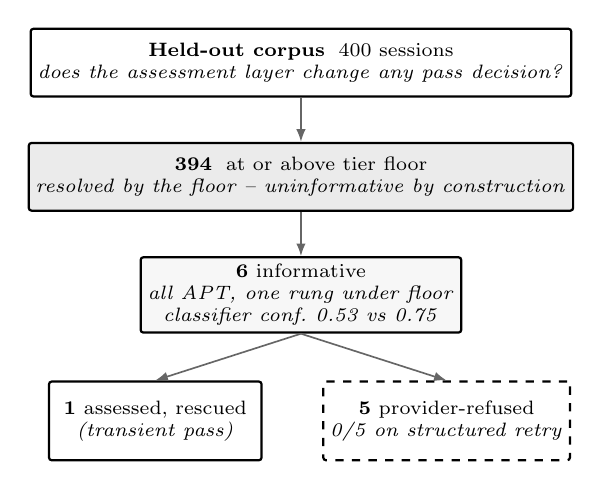
\begin{tikzpicture}[
  font=\scriptsize,
  stage/.style={draw, rounded corners=1pt, thick, align=center,
                inner sep=2.5pt, minimum height=8.6mm},
  dead/.style={stage, fill=black!8},
  live/.style={stage, fill=black!3},
  resc/.style={stage, minimum height=10mm},
  refu/.style={stage, minimum height=10mm, dashed},
  arr/.style={-{Latex[length=1.6mm]}, semithick, black!60}
]
  % 1. full corpus
  \node[stage, minimum width=62mm] (corpus) at (0,0)
       {\textbf{Held-out corpus}\; 400 sessions\\
        \textit{does the assessment layer change any pass decision?}};
  % 2. resolved branch (the inert majority)
  \node[dead, minimum width=50mm] (floor) at (0,-1.45)
       {\textbf{394}\; at or above tier floor\\
        \textit{resolved by the floor -- uninformative by construction}};
  % 3. the informative stratum
  \node[live, minimum width=36mm] (info) at (0,-2.95)
       {\textbf{6} informative\\
        \textit{all APT, one rung under floor}\\
        \textit{classifier conf.\ 0.53 vs 0.75}};
  % 4. live-arm outcomes
  \node[resc, minimum width=27mm] (r1) at (-1.85,-4.55)
       {\textbf{1} assessed, rescued\\ \textit{(transient pass)}};
  \node[refu, minimum width=27mm] (r5) at (1.85,-4.55)
       {\textbf{5} provider-refused\\ \textit{0/5 on structured retry}};
  \draw[arr] (corpus) -- (floor);
  \draw[arr] (floor) -- (info);
  \draw[arr] (info.south) -- (r1.north);
  \draw[arr] (info.south) -- (r5.north);
\end{tikzpicture}
\caption{The fold-down evidence funnel (census in
Table~\ref{tab:hardsunset}). Deterministic routing resolves 394 of 400
held-out sessions at the tier floor before the assessment layer is
consulted; the six sessions below floor form the only stratum where the
top rung can change a pass decision, and the live arm's evidence there
is one transient rescue and five provider refusals that did not recover
on a structured retry.}
\label{fig:funnel}
\end{figure}

The availability result strengthens the removal on its own terms: a
rung that returns empty precisely on APT-shaped sessions is a liability
on the highest-stakes traffic, independent of what its accuracy would
be when it answers.

\begin{table}[t]
\centering
\caption{Fold-down hard-subset census (the released
\texttt{jev\_hard\_subset.json}). The informative stratum for the routing
comparison is the set of held-out sessions whose deterministic routing
lands below the tier's risk floor; on every other row the assessment
layer cannot change the pass decision by construction. The live arm
assessed one of six informative sessions; the other five were refused
by the provider and did not recover on a structured retry protocol
(see text).}
\label{tab:hardsunset}
\small
\setlength{\tabcolsep}{4pt}
\begin{tabular}{@{}lc@{}}
\toprule
Census over the full held-out corpus & \\
(400 sessions) & \\
\midrule
Floor at or above tier floor & 394 \\
Informative (baseline below floor) & 6 \\
\quad tier & all APT \\
\quad under-floor depth & 1 rung \\
\quad classifier conf.\ (inf.\ / corpus) & 0.53 / 0.75 \\
\midrule
Live assessment arm (6 sessions) & \\
\midrule
Assessed and rescued (transient) & 1 \\
Unavailable; 0/5 recovered on structured retry & 5 \\
\bottomrule
\end{tabular}
\end{table}

\emph{Deception effect in closed loop.} Paired closed-loop replays pit a
simulated LLM attacker against the deception engine with and without
kind-aware guidance (\path{jev_dwell_replay_llm_REPORT.md}; 97.8\%
LLM-backed gateway calls, verified by a canary echo probe after an
earlier run was found to have silently template-fallen back). Bait
markers surfaced to the attacker rose from 4 to 9 (+125\%) across the
five error-free family pairs -- a lexical count over five pairs, no
power, direction only. Dwell did not move: 34 vs.\ 33 total turns
in the clean paired comparison, where dwell is operationalized as turn
count, not wall-clock time, and the paired delta is $-1$ turn --
indistinguishable from noise, so the correct reading is a
power-limited null, not an established zero. The report's own mechanism analysis
explains the null: in both arms, nearly every early leave cites
inconsistent fictional filesystem state -- a cautious attacker reads
inconsistency as a trap signal, so response consistency, not deception
style, is the binding constraint. This is precisely why the fiction
graph and verifier sit below the adaptive layer in the ladder: the
consistency rungs are load-bearing for every rung above them.

\emph{Takeaway: the top rung buys assessment coverage and bait exposure,
not dwell time -- and its routing contribution, unresolvable at the
benchmark's ceiling and unavailable on the rows that matter most, was
compiled down to a deterministic floor. The counter-signal is stated
with equal weight: on the 13 real-log sessions, the deterministic floor
misjudged every severity (0/13 at expert level) while the assessed rung
corrected 12 -- the synthetic ceiling and the real-log collapse are the
domain-shift gap in both directions, and they are exactly why the
removal claim is bounded to this benchmark rather than generalized. The
clearest signal in this
evaluation about where intelligence belongs is also the one stated with
its resolution bound.}

\subsection{Scorer-Validity Audit: Manual Annotation of the CTI
Channels}
\label{sec:scorer-audit}

Every deterministic rubric above is itself a measurement instrument,
and the evaluation's conclusions are only as good as its worst
instrument. We therefore audited the two CTI channels against manual
annotation. The full 218-query workload was re-collected with served
text and analysis records persisted per row, packaged into blinded
packets (opaque row identifiers, seeded shuffle, no gold labels, no
pipeline scores), and labeled by two independent annotators ---
fixed-identity open-weights models behind the same runner, standing in
for the independent human raters of the release plan, who receive the
identical packets (\path{results/cti_audit_human_packet/}) --- with a
third annotator adjudicating disagreements. The taxonomy is pinned to
\attck{} Enterprise v19.1 (vendored STIX bundle, sha256-locked, alias
tables for actor normalization); one workload gold label was flagged by
the annotators (an actor alias collision) and is persisted as a quality
flag rather than silently resolved.

The annotators agree with each other at $\kappa = 0.866$ on technique
identification, and their disagreement is almost entirely within
technique families: strict set-F1 is 0.73 for both annotators while
family-level F1 is 1.000 for both (Table~\ref{tab:cti-audit}).
Adjudication resolved every disagreement. The analysis channel is
validated: adjudicated human identification agrees with the machine's
verdicts at $\kappa = +0.75$ (TPR 0.992) --- the Don channel's 0.960
and 0.850 averages measure real extraction, not scorer artifacts.

The served-text channel did not survive its own audit. On technique
rows, every machine-identified/human-rejected conflict --- 67 of the 71
machine-positive verdicts --- has one mechanical cause: the served text
is a deterministic fallback template that echoes the attacker's query
verbatim, and the query contains the technique identifier, so the
string rubric credits error text. The same mechanism explains the actor
suite (all 33 machine-positive verdicts are echoes). Echo-guarding the
scorers --- a re-score of 0 when the response echoes the query verbatim
inside a fallback-shaped surface, matching how every annotator labeled
these rows --- collapses the audited surface's served-text means from
0.524 to 0.057 (technique) and 0.680 to 0.000 (actor), and
machine-vs-human agreement rises from $\kappa = -0.19$ to $+0.35$
(technique) and from $0.05$ to $0.91$ (actor): the guarded machine now
agrees with the human labels it previously contradicted.

Because the audited surface was proven row-identical to the current
configurations' re-runs (pre-guard score equality on all 218 rows), the
guarded numbers above are the corrected values for the released
two-channel artifact (Table~\ref{tab:two-channel}). The September
campaign surface is different, and we recompute rather than assume: on
the campaign's persisted response previews, 61 of 123 technique rows
and 25 of 35 actor rows are echo templates, and the guarded,
served-text-only means --- computed on previews truncated at 200
characters, hence lower bounds --- are $\geq 0.107$ (technique) and
$\geq 0.163$ (actor), against raw both-channel figures of 0.960 and
0.850. Three properties of this evaluation are unchanged by the
correction, and none depends on a string rubric: the
zero-unverified-serves result and the verifier's red-team precision and
recall; every paired per-row delta in the external-baseline ladder,
whose compared arms serve byte-identical strings; and the analysis
channel itself. What the correction removes is the claim that the CTI
suites' \emph{served} text carried the expected intelligence on this
infrastructure: under free-tier generation the served surface for those
suites was substantially deterministic templates, the analysis channel
carried the value, and the two-channel declaration --- adopted before
the audit --- is what kept the two findings separable. The persona
suite is untouched: its scorer already penalized echoes, its 60 rows
score identically raw and guarded (0.649), and its quality evidence is
the judge-panel consensus study, not a string rubric.

% Auto-generated by scripts/gen_two_channel_tables.py — 2026-09-28
% Declared scoring channels (never mix without labeling):
%   served_text  = deception realism (what the attacker receives)
%   cti_analysis = intelligence value (Don extraction; NOT served)
% Served-text numbers are echo-guarded (blinded-audit correction,
%   results/cti_manual_audit.json); the audited surface was proven
%   row-identical to the two-channel reference run (218/218 pre-guard score equality).

\subsection{Two-Channel Evaluation}

Every metric below declares its \emph{scoring channel}. The \textbf{served-text} channel scores what the attacker actually receives; the \textbf{CTI-analysis} channel scores what the pipeline identified (Don extraction), which is never shown to the attacker. The two answer different questions---deception realism vs.\ intelligence value---and are never combined into a single composite.

The served-text rubric originally credited a technique identifier or actor name appearing anywhere in the response. A double-annotated blinded audit (\S\ref{sec:scorer-audit}) found that on fallback-heavy runs the served surface is dominated by deterministic templates that echo the query verbatim, so the raw rubric credited error text (97 of 218 rows corrected). Both raw and guarded columns are shown: the gap itself is a finding about the serve surface.

\begin{table}[t]
\centering
\caption{Two-channel metrics of the verified RAGIN pipeline (generator: gateway default (glm-5.3-flash-free)). Served text is shown raw (the echo-crediting rubric) and echo-guarded (post-audit); the guarded column is canonical. The deception surface deliberately answers CTI-style questions with machine transcripts, not technique essays; the intelligence value lives in the analysis channel. Guarded numbers are computed on the audited surface, proven row-identical to this run by pre-guard score equality on all 218 rows (\texttt{cti\_manual\_audit.json}).}
\label{tab:two-channel}
\begin{tabular}{lccc}
\toprule
Suite & Served (raw) & Served (guarded) & CTI analysis \\
\midrule
Technique identification (123 q) & 0.524 & 0.057 & 0.960 \\
Actor attribution (35 q) & 0.680 & 0.000 & 0.850 \\
Persona realism (60 q) & 0.649 & 0.649 & -- \\
\bottomrule
\end{tabular}
\end{table}

\begin{table}[t]
\centering
\caption{External baselines on the 218-query workload (generator: deepseek-v4-flash-free for all LLM arms). \textbf{All scores are served-text channel under the raw (pre-guard) rubric}---the deception quality an attacker experiences. Paired per-row deltas are scorer-invariant: the verified loop serves byte-identical strings to the no-verifier arm on all 218 rows (paired delta 0.000), and the host-fiction layer adds cross-session consistency at exactly zero quality cost (paired per-row delta 0.000). Absolute levels on fallback-heavy runs shift under the echo guard (Table~\ref{tab:two-channel}); the grounding and consistency contrasts do not.}
\label{tab:baseline-served-text}
\begin{tabular}{lc}
\toprule
Arm & Served-text composite \\
\midrule
Vanilla Cowrie (no LLM) & 0.001 \\
Stateful LLM (HoneyGPT/LLM-SSHH) & 0.070 \\
Bare LLM (unverified) & 0.502 \\
RAGIN w/o verifier & 0.618 \\
RAGIN full (verified loop) & 0.618 \\
RAGIN full + host fiction & 0.618 \\
\bottomrule
\end{tabular}
\end{table}

\begin{table}[t]
\centering
\caption{Blinded annotator audit of the automated scorers (\S\ref{sec:scorer-audit}): two independent blinded annotators (fixed-identity free-tier models, no gold labels, no pipeline scores), third-annotator adjudication, taxonomy pinned to \\attck{} Enterprise v19.1 (vendored STIX, sha256-locked). Scorer-vs-annotator agreement is Cohen's $\kappa$ between the automated channel verdicts and the adjudicated annotator labels, before/after the echo guard. All disagreements were adjudicated; none unresolved.}
\label{tab:cti-audit}
\small
\setlength{\tabcolsep}{3.5pt}
\begin{tabular}{@{}lccccc@{}}
\toprule
Suite & $n$ & $\kappa$ (A,B) & strict F1 (A/B) & adjud.\ A/B/neither & scorer-vs-annot.\ $\kappa$ pre$\to$post \\
\midrule
Technique identification & 123 & 0.866 ($n$=123) & 0.732/0.732 & 4/3/0 & -0.187$\to$0.349 \\
Actor attribution & 35 & 0.160 ($n$=35) & 0.771/0.765 & 2/4/0 & 0.048$\to$0.914 \\
Persona realism & 60 & 0.072 ($n$=60) & --/-- & 4/8/4 & 0.099$\to$0.099 \\
\bottomrule
\end{tabular}
\end{table}

% Echo-guard correction provenance: results/cti_manual_audit.json (echo_guard_correction): 97 rows changed; served avg pre->post: technique 0.5236->0.0569, actor 0.68->0.0, deception 0.6492->0.6492 (persona scorer already penalized echoes). Post-guard scorer-vs-annotator kappa: technique -0.187->+0.349, actor 0.048->0.914 (scorer now agrees with the annotator models). Ladder paired per-row deltas are scorer-invariant (byte-identical served strings across compared arms on the decisive rows).

% Historical note (Sep-22 campaign): its official technique (0.960) and actor (0.850) averages were BOTH-channel (served text max analysis). Its served-text-only equivalents are 0.493 / 0.666 under the raw rubric. Do not compare across channels; see results/technique_rubric_diff_investigation.json.


\subsection{Run-to-Run Stability}
\label{sec:stability}

LLM-driven systems rarely report whether their numbers replicate, so we
ran the full 218-query campaign twice, independently, with identical
configuration (Figure~\ref{fig:results}, bottom). The composite moves
from $0.880$ to $0.884$ ($\Delta
+0.005$); per-row pass-decision agreement is $0.991$ (216 of 218 rows).
The deterministic strata reproduce exactly (technique and actor suites:
per-row mean absolute difference $0.000$); the persona stratum, the only
LLM-judged stratum, shows MAD $0.096$ with pass agreement $0.967$. The
headline metrics are identical across runs: 132 TTPs, 67 unique,
218/218 engagement, 218/218 persona assignment. This is the signature we
want: scored-deterministic claims reproduce deterministically, and the
only variance is bounded judge sampling noise.

Recomputed on the judge-audited rows of the previous subsection
(\path{stability_run1_vs_run2.json}, audited panel), the
comparison is unchanged: the audited composite moves $0.883\to0.888$
($\Delta+0.005$, artifact values 0.8826 and 0.8877) with the same $0.991$ pass
agreement, and the audited
deception suite shows MAD $0.097$ with agreement $0.967$. The audited
figures reconcile exactly with the raw ones: only the 60 persona rows
differ (one reclassified harness row, one bait-credit row, rounded
floats), and the audited suite means retain the reclassified harness
row at its recorded 0.0 -- the deception-only means excluding harness
artifacts, $0.756$ and $0.762$, are persisted alongside rather than
chosen silently. Two facts are
worth recording. First, the run-to-run variance is generator-side: 32
of 60 persona rows differ between runs, only one of them touched by the
audit, so the MAD's variance comes from provider sampling, not judge
error. The scorer audit adds a caveat the raw agreement conceals: on
the CTI suites the two runs' per-row score equality is
template-assignment determinism, not content determinism -- under the
echo guard the two runs' guarded served-text means separate (0.479
vs.\ 0.455 technique, computed on persisted previews) -- so the
deterministic-strata reproduction claim, true of the recorded scores,
must not be read as transcript identity. Second, both raw and audited comparisons carry the same
verdict (stable) in the persisted artifact, so no narrative choice
between them changes the stability conclusion.

\subsection{Threats to Validity}
\label{sec:threats}

\emph{Construct.} Suite scores reward grounded technique coverage; a
system could game them by keyword stuffing. The persona rubric and the
judge-panel consensus study exist partly to catch exactly that failure,
and the two agree --- and the echo-credit failure the manual audit
caught (\S\ref{sec:scorer-audit}) is precisely this defect class,
realized not by an adversary but by the system's own fallback path; the
guarded scorers, the audit artifact, and the raw-vs-guarded columns of
Table~\ref{tab:two-channel} now bound it. \emph{Internal.} The judge model shares a provider with the generator (different family); the consensus protocol, rubric
corrections, and the deterministic strata bound but do not eliminate
provider-common-mode effects, and the judge panel is one model however
partitioned, so the quality study has no inter-judge or human
component. The rubric corrections were derived and applied on the same
corpus. \emph{External.} The deployment observes tailnet traffic only: no ambient internet background
radiation, no botnet churn, no real APT dwell time; the live fleet runs
one SSH listener plus HTTP and Telnet services on the same session
interface, so web-shaped attack surfaces in particular are
under-represented. The workload personas approximate
but do not replace live adversaries, and the consensus study's
evaluators, however adversarial, are models. The routing corpus is
synthetic and the floor's patterns were tuned against its generator, so
the fold-down ceiling is in-sample for the tuning process; the 13-session
real-log study points the other way and is too small to resolve.
\emph{Statistical.}
Bootstrap CIs are computed over paired rows (percentile, 10{,}000
resamples, fixed seed); Wilson intervals are used for pass rates;
scenario counts per suite
(35--123) bound interval width, which we report rather than
over-claiming. The RQ4 comparisons are power-limited throughout (13
real-log sessions, five replay pairs, six informative census rows, ten
steering predictions) and are priced as directional evidence, not
established effects. No external baseline was run at the
version-of-record workload: the comparisons are the loop against its
own ablations, which prices mechanisms within the architecture but
cannot price the architecture against practice. A preliminary external
comparison exists in the released tree (\path{cowrie_comparison.json},
July 2026): 30 sessions of the pre-campaign benchmark against 2
sessions from a live Cowrie deployment (composite 0.697 vs.\ 0.45;
RAGIN covers all TTPs the Cowrie corpus observed). We report it as
directional only -- its sample is orders of magnitude too small and its
workload predates the campaign of this section -- but it establishes
that the harness runs against a traditional baseline without
modification. A full external baseline on the version-of-record
workload (vanilla Cowrie, a stateful LLM, an unverified LLM, and
RAG-without-verifier variants, generator-held-fixed) now exists in the
released tree (\path{external_baseline_model_coherent.json},
Table~\ref{tab:baseline-served-text}); its paired per-row deltas are
the durable content, while its CTI-suite absolute levels are
fallback-dominated and are reported raw under the declared served-text
channel with the guard analysis of \S\ref{sec:scorer-audit} applied
where the persisted surface allows. What remains open is the guarded
regeneration of the CTI suites on a healthy-generation window with
full-transcript persistence --- the field campaign's collection path
now persists both.

\section{Discussion}
\label{sec:discussion}

\subsection{What the Loop Buys, What the Ladder Prices, and What Neither Can}
The verified loop replaces confidence in the generator with an audited
pipeline, and the evaluation localizes what each stage
contributes. The ladder adds the accounting: which rungs of intelligence
carry measurable weight. The RQ4 results cut both ways -- the
grounding rung is load-bearing, while the top rung's routing benefit
was not resolvable above the deterministic floor -- and the rung's
provider refused assessment precisely on the highest-stakes sessions --
so the LLM came out of that path. The loop makes spent intelligence
safe; the ladder keeps it cheap. Neither makes the provider problem
disappear, and the hard-subset census adds a wrinkle: the free-tier
endpoint intermittently refuses security-shaped payloads outright
(HTTP 403 on attacker-tooling states, benign states served). For a
deployment whose critical moments are attack-shaped, provider refusal
is not only a cost risk but a selective availability risk concentrated
exactly where assessment matters most. Every
generative claim in this paper is downstream of a free-tier inference
API: the safety-alignment timeouts that shaped the persona stratum, the
catalog churn the watcher caught, and the quota windows that gated the
study schedule are all the same structural fact. We treat the provider as
an unreliable component and the system degrades safely when it fails, but
a practitioner sizing a deployment should budget for generation being
\emph{eventually unavailable} in exactly the way the fallback path
assumes -- and should read the fold-down rule as the remedy: every
mechanism compiled down to a certifiable equivalent is one fewer
dependency on that provider.

\subsection{Deployment Guidance}
Five lessons from operating the system generalize. First, run the
watcher: provider catalogs drift, and a wired model disappearing silently
is a production incident for any LLM-dependent defense. Second, scope the
HITL gate with care: the gate exists for content classes whose
compromise value is high, and the audit log it produces doubles as the
governance record. Third, keep the deterministic floor maintained: the
fallback transcripts are load-bearing. The system is only as consistent
as its last vetted transcript, and treating those transcripts as second-class
content would hollow out the safety property that makes the LLM path
permissible. Fourth, budget for provider instability as a first-class
operating condition: during this study the watcher logged one wired model
disappearing from the catalog and one quota-exhaustion window, and the
fallback path absorbed both without serving unverified content; the
watcher's probe history also records an unwired catalog model appearing
in and vanishing from the listing between consecutive twice-daily
probes -- churn the serving path never touched because nothing was
wired to it. An
LLM-dependent defense sized without that budget will be sized wrong.
Fifth, audit the ladder on a schedule: re-price each intelligent rung
against its cheapest certifiable competitor as the deterministic
machinery matures. In this study the audit already paid out once --the kind-aware routing rung was removed after deterministic fixes reproduced
its accuracy on the benchmark -- while the same rung's 12/13 record on
thirteen real-log sessions (against the floor's 0/13) is the standing
caveat on that removal -- leaving the serving path with one fewer model,
provider, and failure mode -- and in the released system the audit is
not a manual exercise: the judge-panel audit and audited stability
reseed automatically whenever a new campaign run lands (Appendix~\ref{app:audit}).

\subsection{Cost and Practicality}
A defender considering this architecture is entitled to ask what it costs.
The serving host is a commodity box (2~vCPU, ${\sim}4$~GB RAM) shared with
the honeypot listeners; profiling adds milliseconds per session, retrieval
over the curated corpus adds tens of milliseconds, and the dominant cost
is provider inference, bounded per draft by output caps and low
temperature. The mean session in the live campaign completed in
${\sim}44$~s end to end, dominated by the generative turns, and the
deterministic strata served in fractions of a second. The economically
interesting number is the fallback rate: when the provider refused or
timed out, the loop degraded to vetted transcripts rather than
open-ended retries, so the cost ceiling per session is two generative
attempts plus one deterministic serve. On a free-tier allowance the full
218-query campaign completes within a daily quota window, which is the
difference between a system a lab can operate and one it cannot.

\subsection{Generalizing the Ladder and the Loop}
Nothing in the loop is specific to honeypots, and neither is the ladder.
The shape, generate under
grounded context, verify the draft against a persisted state structure,
serve only on pass, fall back to vetted content on failure, applies
wherever an LLM writes output whose downstream consumer is adversarial or
safety-critical: SOC copilot drafting incident narratives, retrieval
chatbots answering from a curated corpus, agent pipelines writing into
structured stores. The fiction graph generalizes to any \emph{state
bound} the LLM must respect; the verifier to any checkable draft
property; the deterministic fallback to any canned-but-correct content.
The certifiability axis is the portable part of the ladder: any
mechanism in any such pipeline can be placed on it, priced by marginal
effect, and audited for fold-down as certifiable alternatives mature.
The evaluation here does not establish that the
pattern transfers, but the
architecture section is written so that a practitioner in another domain
can lift the loop wholesale, and the ablation battery (A1--A5) plus the
RQ4 pricing protocol are the template for testing whether each piece
they keep contributes.

\subsection{Ethics}
The system deploys deception against real attackers, which obligates
care. All credential material shown to attackers is registered canary
secrets: nothing real is ever exposed, and any canary appearing in
outbound traffic is attributable to bait interaction by construction. The
HITL gate keeps a human decision between the system and the highest-stakes
content classes, and the append-only audit log records every gate
decision. The testbed is isolated from production networks, and the
deception targets only actors actively attacking it. The 13 replayed
real-log sessions come from the project's own Cowrie captures of
traffic against the isolated testbed; they contain no production
credentials and are released only in feature form (command sequences,
family labels), not as raw transcripts. One dual-use consideration is
stated rather than left implicit: the release includes the verifier's
decision procedures and the scenario sets, so an attacker who studies
them knows exactly which consistency surface is enforced and can craft
probes against the extraction layer's recall; we judge the reproduction
value of the release to outweigh this, but the surface is now declared.
We release scenario
sets and scoring harnesses so that the community can audit the
evaluation, not just the code.

\subsection{Limitations}
The deployment observes tailnet traffic only; the ambient-internet axis
(scanners, botnets, opportunistic ransomware) is absent by design choice
and limits ecological claims. The consensus study's three evaluator
personas share one judge model family; multi-model judging failed on the
provider at study time (a listed model returned 404 on real calls despite
catalog presence), a gap we flag for the watcher's future checks. No
human raters participated; the study is an LLM-judge panel, and a small
expert-rater pass over the eight released transcripts is the direct
remedy we name as required future work. The
$0.750$ agreement figure should therefore be read as within-model
consistency -- how stably one model's prompted personas concur -- rather
than inter-annotator agreement across independent judges. The shell-scope listener constrains web-shaped deception scenarios, as the
weakest consensus scenario illustrates. And the persona-realism stratum,
while stable run-to-run, remains the stratum where judge variance lives;
its scores should be read with the MAD in \S\ref{sec:stability} in mind.
The RQ4 evidence carries its own weight limits: the real-log assessment
sample is 13 sessions, the closed-loop replay pairs number five
clean families, and the simulated attacker, however instrumented, is not
an adversary with a stake in the outcome. The routing fold-down rests on
200 held-out sessions at ceiling plus a full-corpus census locating the
informative stratum (six sessions, one rescued live, five lost to
provider refusals); it is stated at the benchmark's resolution rather
than as general subsumption. The deception-effect claims for the
top rung (bait exposure, the dwell null) are directional, and we price
them as such rather than as established effects.

\section{Related Work}
\label{sec:related}

\subsection{Honeypot and Honeynet Architectures}
Deception research has moved from single-service traps to orchestrated
honeynets~\cite{spitzner2002}, with recent surveys cataloging managed
deception fabrics and cloud-native deployment~\cite{lopez2024}. Multi-sensor
platforms aggregate dozens of low- and medium-interaction sensors in one
stack, and containerized honeynets scale the same idea
elastically~\cite{t-pot2024}. The survey's gap analysis is blunt: no
widely deployed framework grounds its responses in real-time threat
intelligence or differentiates behavior across attacker classes, which
are the two capabilities G1 and \S\ref{sec:chrollo} exist to provide.
What these architectures share is a static
relationship between the decoy and its content: the deception is authored
once, at deployment time. \system differs in kind, not degree: its served
content is decided per session, and every decision passes a verification
gate before reaching the wire.

\subsection{Generative Models in Deception}
LLM-backed honeypots are the closest line of work, and the field has
moved quickly from feasibility demonstrations to state-aware designs.
GPT-driven SSH bots demonstrate that language models can hold convincing
interactive sessions~\cite{kouremetis2024}; LLM-generated web deception
serves convincing HTTP responses for arbitrary paths~\cite{galah2024};
RAG-coupled generation grounds responses in retrieved
content~\cite{qiao2025,sezgin2025decoypot}, and agentic RAG pipelines
have been proposed for CTI workflows~\cite{belmahjoub2025,gao2025}.
HoneyGPT breaks the classical flexibility/depth/deception trilemma with
structured prompting and reports a three-month field
evaluation~\cite{wang2026honeygpt}; DecoyPot drives a web-API honeypot
with a RAG agent improved from live attacker
traffic~\cite{sezgin2025decoypot}; and LLMHoney pairs a virtual file
system with real-time LLM response generation~\cite{malhotra2025llmhoney}.
Most directly relevant to this paper's machinery, a 2026 generation of
systems now treats state and validation explicitly: LLM-SSHH serializes a
persistent state snapshot into the prompt and validates generated
responses against state constraints, rejecting hallucination-driven
inconsistencies~\cite{li2026llmsshh}, and GenPot couples generative
interaction across command-line, API, and web surfaces with state
management and guardrails, evaluated operationally and at
scale~\cite{laragutierrez2026genpot}. A recent SoK systematizes this
design space and its failure modes~\cite{bridges2026}.

The gap this paper addresses is therefore no longer whether LLM honeypots
can be consistent -- the newest systems demonstrate exactly that -- but
what the consistency machinery is \emph{for}. Prior systems improve or
validate generative consistency: state snapshots and constraint checks
(LLM-SSHH), guardrails and state management (GenPot), structured
prompting (HoneyGPT) are mechanisms for making the generator's output
stay believable. This work turns the entire serving path into an
explicitly verified security architecture: every response is either
admitted by a serving-time verifier against a session-scoped fiction
graph with a recorded verdict, served from human-vetted deterministic
content, or withheld -- with the verifier itself red-teamed by labeled
cases and live-LLM-authored drafts (\S\ref{sec:rq2}) -- and every safety
decision lands in an append-only audit trail a human gate can act on
(G3, G5). The second difference is methodological and, we argue, the
paper's central contribution: the intelligence-ladder evaluation places
every mechanism on a certifiability axis and prices each rung by measured
marginal effect, including the fold-down direction -- an adaptive rung
whose benefit a certifiable mechanism reproduces is removed from the
serving path (\S\ref{sec:jeveval}). Prior systems argue \emph{for} their
intelligent components; this evaluation is designed to argue
\emph{against} them and to keep only what survives pricing.
Table~\ref{tab:related-matrix} summarizes the positioning along the
dimensions this paper treats as first-class security properties.

\begin{table*}[t]
\centering
\caption{Positioning against recent generative-honeypot systems. Y =
present as a first-class, evaluated mechanism; P = partial (mechanism
present but not evaluated under adversarial pressure, or scoped to
response content only); N = not reported. Entries reflect the cited
papers' own evaluations; where a capability is absent from a paper's
reported design we mark N without implying the system could not add it.
\system's column is the only one whose evaluation includes a priced
fold-down of an intelligent component.}
\label{tab:related-matrix}
\small
\setlength{\tabcolsep}{3.4pt}
\begin{tabular}{lccccccccc}
\toprule
 & \rotatebox{60}{State consistency} & \rotatebox{60}{Serving-time verification} & \rotatebox{60}{Danger/safety gate} & \rotatebox{60}{Deterministic fallback} & \rotatebox{60}{CTI grounding} & \rotatebox{60}{Human-in-the-loop gate} & \rotatebox{60}{Verifier red-team} & \rotatebox{60}{Field deployment} & \rotatebox{60}{Mechanism fold-down} \\
\midrule
HoneyGPT~\cite{wang2026honeygpt} & P & N & N & N & N & N & N & Y & N \\
DecoyPot~\cite{sezgin2025decoypot} & P & N & N & N & Y & N & N & N & N \\
LLMHoney~\cite{malhotra2025llmhoney} & P & N & N & P & N & N & N & N & N \\
LLM-SSHH~\cite{li2026llmsshh} & Y & P & N & N & N & N & N & N & N \\
GenPot~\cite{laragutierrez2026genpot} & P & P & P & N & N & N & N & P & N \\
\system (this work) & Y & Y & Y & Y & Y & Y & Y & P & Y \\
\bottomrule
\end{tabular}
\end{table*}

\subsection{LLM Security and Alignment Pressure}
Our provider-fragility observations connect to a broader alignment literature.
Safety-aligned models refuse or deflect on adversarial-role prompts, and
constitutional and RLHF training shapes exactly the refusal behavior our
harness must route around~\cite{bai2022,ganguli2022,christiano2017}.
Prompt-injection risks in retrieval pipelines motivate the corpus hygiene
of \S\ref{sec:implementation}~\cite{greshake2023,perez2022}, and
documented failures of ML-backed security tooling under distribution
shift~\cite{reworr2024} reinforce the case for measured fallbacks over
trusting generation. The generate-then-check pattern itself has
classical roots, and modern guardrail and safety-filtering systems
structure the same draft-then-verify separation around content policy
rather than world-model consistency~\cite{inan2023}; our verifier
differs in checking against a session-scoped fiction the defender fully
controls, which makes the check a decision procedure rather than
another learned judgment. The deployment lesson we add is operational:
treat the provider as an unreliable component with catalog drift, quota
exhaustion, and alignment-induced timeouts as normal operating conditions.
The reviewer-facing implication is a methodological one: evaluations of
LLM-driven defenses should report provider instability as part of the
results, because it shaped which experiments were even runnable.

\subsection{CTI and Behavior Analysis}
Hybrid RAG over threat intelligence has been shown effective for
attribution and technique mapping~\cite{alsada2024,rajapaksha2024},
agentic RAG for attack investigation and incident
response~\cite{blefari2025,liu2025}, and TTP extraction from unstructured
text predates the current generation of systems~\cite{orbinato2022}.
RAG-driven deception in the honeypot context specifically is represented
by DecoyPot's self-improving RAG agent~\cite{sezgin2025decoypot} and
adaptive RAG honeypot architectures~\cite{qiao2025}; what these systems
ground is response content, whereas this paper's retrieval rung grounds
the \emph{plan} (which facts to project, which bait to attach to which
predicted technique) and its effect is measured by a paired ablation with
a structural-dependence control (\S\ref{sec:rq1}).
Behavioral profiling of attacker sessions underpins both intrusion
detection~\cite{bachl2021,farasat2024b,sharafaldin2018} and
honeypot-facing classification~\cite{lekssays2025}, and attack-graph
sequence models connect observed actions to
attribution~\cite{alsaheel2021,noureddine2020}. Adaptive
deception experiments show that attacker skill modulates effective
strategy~\cite{kouremetis2024,jeon2024}, and honeytoken-based
attribution~\cite{spitzner2003,valeros2024} motivates the
canary-registered bait
design. \system composes these primitives into a loop whose safety
properties, rather than its raw capability, are the contribution.

\section{Conclusion}
\label{sec:conclusion}

Honeypots have spent two decades recording attacker behavior without
reasoning about it, and the arrival of generative models promised to close
that gap while opening a worse one: a deception tool whose product is
unverified improvisation. This paper argued that the right unit of design
is not the generator but the \emph{loop} around it. \system couples
behavioral profiling, retrieval-grounded planning, a fiction graph, and
serving-time verification into a cycle in which every response is either
verified against the session's deception state or served from vetted
deterministic content, with a human gate on the highest-stakes material
and an audit trail over every decision.

The evaluation supports the division of labor the architecture claims,
and the escalation analysis prices it rung by rung. Retrieval grounding
is the rung the system cannot lose: removing
it costs $+0.154$ composite ($[+0.092, +0.221]$) under rubrics scored
identically in both arms, and the raw detection count collapses to zero
with it -- a structural dependence, reported as such
(\S\ref{sec:rq1}) -- while leaving persona realism untouched, a null
result the design predicts.
The fiction graph and verifier maintain their properties under targeted
adversarial pressure: zero contradictions across 45 re-queries, zero
unverified serves across a 218-query live campaign, an induced-failure
census showing the checks do reject, and an ablation
battery in which each mechanism's removal costs the property it was added
to provide. The deception holds a three-persona LLM-judge consensus of
$3.86/5$ with
$0.750$ exact agreement across personas of one judge model -- a
within-model consistency measure rather than inter-annotator agreement,
and not a human evaluation
-- and two independent full campaigns reproduce the
composite to $+0.005$ with the deterministic strata replicating exactly.
At the top of the ladder, the result is a subtraction with a standing
caveat: kind-awareness fixed 12/13 real-log assessments (against the
deterministic floor's 0/13 on the same sessions) and lifted bait exposure
by 125\%, added no measurable dwell time, and showed no marginal routing
effect that the benchmark could resolve -- so it left the serving path,
with the domain-shift gap the real-log study exposes named as the
caveat on that removal.
Each rung we retained paid for itself in its measured contribution, and
the rung we removed is the result that carries furthest beyond this
system -- bounded to the benchmark that measured it.

The limits are stated with the same directness. The deployment hears no ambient
internet; the judge shares a provider with the generator; and the
availability of generative components is structurally hostage to provider
quota and alignment posture, a constraint the fallback path absorbs but
does not remove. None of these limits is hidden by the loop; all of them
are measured by it. We release the scenario sets, the scoring harnesses,
and every persisted artifact behind the numbers in this paper -- code,
cloud stack, results, and the compiled paper itself -- at
\url{https://github.com/0xzodiac/The-Intelligence-Ladder}, so that the
claims can be replayed rather than believed.

We see four directions as the most productive next steps. First, extending the fiction
graph across sessions, so that the longitudinal attacker memory and the
consistency machinery stop being separate systems and cross-session
deception inherits cross-session verification. Second, broadening the verifier red-team
evaluation: the released induced-failure harness now covers both
strata -- 96 canonical cases at the deterministic stratum (precision
and recall 1.000) and 497 live-LLM-authored drafts from two author
models across seven iterative rounds (final precision 1.000 on both
authors, recall 0.931/0.943, zero false positives) -- its 23
distinct verifier findings, including three live false-positive
roots, are fixed and regression-locked, and the harnesses themselves
are the deliverable: a sequenced third-author plan (different model
family, documented budget and falsifiable expected deltas) ships with
the artifacts so the next iteration is an execution, not a design
exercise. Multiturn injection chains and a sampled manual audit of
campaign-scale TTP extractions remain open. Third, field evaluation on
internet-reachable deployments, where the ambient-traffic axis this
testbed excludes by scope choice becomes measurable, and the steering
hypothesis, better bait, measurable attacker dwell, can be tested against
adversaries who did not consent to be studied; the same field cycle
should add an external-baseline comparison (vanilla Cowrie, an
unverified LLM honeypot) on shared metrics and a small human-rater
study over the released transcripts. Fourth, treating the ladder
audit as an ongoing protocol: as the deterministic machinery matures,
each intelligent rung should be re-priced against its cheapest
certifiable competitor, and the loop should shrink accordingly. The
system this paper releases is one where that audit has already run once,
and the serving path is smaller because of it.


\begin{IEEEbiographynophoto}{Anonymous}
is with the Department of Computer Science, Benha University, Egypt. His
research interests include cyber deception and honeypot design,
retrieval-augmented generation for security tooling, applied large
language models under verification, and threat-intelligence grounding of
autonomous defense systems.
\end{IEEEbiographynophoto}

\begin{thebibliography}{40}

\bibitem{alsada2024} B. Al-Sada, A. Sadighian, and G. Oligeri, ``Analysis and Characterization of Cyber Threats Leveraging the MITRE ATT\&CK Database,'' \emph{IEEE Access}, vol.~12, pp.~1217--1234, 2024.

\bibitem{bachl2021} M. Bachl, J. Fabini, and T. Zseby, ``A Flow-Based IDS Using Machine Learning in eBPF,'' arXiv preprint arXiv:2102.09980, 2021.

\bibitem{crowdstrike2026} CrowdStrike, ``2026 CrowdStrike Global Threat Report: AI Accelerates Adversaries and Reshapes the Attack Surface,'' CrowdStrike Inc., Threat Intelligence Report, Feb.\ 2026. [Online]. Available: \url{https://www.crowdstrike.com/resources/reports/global-threat-report/}

\bibitem{belmahjoub2025} M. Belmahjoub and L. Benhiba, ``Causal-Aware Knowledge Graph Enhanced RAG for Predictive Cybersecurity Intelligence,'' in \emph{Proc.\ ISCMI}, pp.~136--141, 2025.

\bibitem{ibm2024} IBM Security, ``Cost of a Data Breach Report 2024,'' IBM Corporation, Technical Report, 2024. [Online]. Available: \url{https://www.ibm.com/reports/data-breach}

\bibitem{chaudhari2024} H. Chaudhari et al., ``Phantom: General Backdoor Attacks on Retrieval Augmented Language Generation,'' arXiv preprint arXiv:2405.20485, 2024.

\bibitem{blefari2025} F. Blefari, C. Cosentino, A. Sorbello, and F. Marozzo, ``CyberRAG: An Agentic RAG Cyber Attack Classification and Reporting Tool,'' arXiv preprint arXiv:2507.02424, 2025.

\bibitem{orbinato2022} V. Orbinato et al., ``Automatic Mapping of Unstructured Cyber Threat Intelligence: An Experimental Study,'' in \emph{Proc.\ ISSRE}, pp.~181--192, 2022.

\bibitem{alsaheel2021} A. Alsaheel et al., ``ATLAS: A Sequence-based Learning Approach for Attack Investigation,'' in \emph{Proc.\ USENIX Security}, pp.~3005--3022, 2021.

\bibitem{noureddine2020} M. Noureddine et al., ``Revisiting ATT\&CK Matrix for Unified Cyber Threat Intelligence,'' arXiv preprint arXiv:2012.09988, 2020.

\bibitem{farasat2024b} T. Farasat, J. Kim, and J. Posegga, ``SmartX Intelligent Sec: A Security Framework Based on Machine Learning and eBPF/XDP,'' arXiv preprint arXiv:2410.20244, 2024.

\bibitem{fayyazi2023} R. Fayyazi, R. Taghdimi, and S. Yang, ``Advancing TTP Analysis: Harnessing the Power of Large Language Models with Retrieval Augmented Generation,'' in \emph{Proc.\ ACSAC Workshops}, pp.~255--261, 2023.

\bibitem{gao2025} X. Gao and X. Chang, ``A Retrieval-Augmented Generation Framework Based on a Knowledge Graph of Cybersecurity Vulnerabilities in Power Networks,'' \emph{IEEE Access}, vol.~13, pp.~186693--186710, 2025.

\bibitem{jeon2024} J. Jeon, J. Koo, and Y. Kim, ``RAG-based Cyber Threat Tracing Graph Modeling Method,'' in \emph{Proc.\ TrustCom}, pp.~608--615, 2024.

\bibitem{jia2025} A. Jia, A. Ramesh, Z. Shamsi, D. Zhang, and A. Liu, ``RAGRank: Using PageRank to Counter Poisoning in CTI LLM Pipelines,'' arXiv preprint arXiv:2510.20768, 2025.

\bibitem{kouremetis2024} M. Kouremetis et al., ``Mirage: Cyber Deception Against Autonomous Cyber Attacks in Emulation and Simulation,'' \emph{Annals of Telecommunications}, vol.~79, pp.~803--817, 2024.

\bibitem{lekssays2025} A. Lekssays et al., ``TechniqueRAG: Retrieval Augmented Generation for Adversarial Technique Annotation in Cyber Threat Intelligence Text,'' in \emph{Proc.\ ACL}, 2025.

\bibitem{lewis2020} P. Lewis et al., ``Retrieval-Augmented Generation for Knowledge-Intensive NLP Tasks,'' arXiv preprint arXiv:2005.11401, 2020.

\bibitem{liu2025} Z. Liu and A. Anwar, ``AutoBnB-RAG: Enhancing Multi-Agent Incident Response with Retrieval-Augmented Generation,'' arXiv preprint arXiv:2508.13118, 2025.

\bibitem{lopez2024} P. B. L\'opez, M. G. P\'erez, and P. Nespoli, ``Cyber Deception: State of the Art, Trends and Open Challenges,'' arXiv preprint arXiv:2409.07194, 2024.

\bibitem{paul2025} S. Paul, F. Alemi, and R. Macwan, ``LLM-Assisted Proactive Threat Intelligence for Automated Reasoning,'' arXiv preprint arXiv:2504.00428, 2025.

\bibitem{qiao2025} Y. Qiao et al., ``SecRAG: A Graph-Enhanced RAG Framework with Dynamic Prompt for Cybersecurity Applications,'' in \emph{Proc.\ CSCWD}, pp.~2053--2058, 2025.

\bibitem{rajapaksha2024} S. Rajapaksha, R. Rani, and E. Karafili, ``A RAG-Based Question-Answering Solution for Cyber-Attack Investigation and Attribution,'' in \emph{Proc.\ ESORICS Workshops}, 2024.

\bibitem{reworr2024} Reworr and D. Volkov, ``LLM Agent Honeypot: Monitoring AI Hacking Agents in the Wild,'' arXiv preprint arXiv:2410.13919, 2024.

\bibitem{roy2023} S. Roy, E. Panaousis, C. Noakes, A. Laszka, S. Panda, and G. Loukas, ``SoK: The MITRE ATT\&CK Framework in Research and Practice,'' \emph{ArXiv}, vol.~abs/2304.07411, 2023.

\bibitem{sharafaldin2018} I. Sharafaldin, A. H. Lashkari, and A. A. Ghorbani, ``Toward Generating a New Intrusion Detection Dataset and Intrusion Traffic Characterization,'' in \emph{Proc.\ ICISSP}, pp.~108--116, 2018.

\bibitem{shinde2020} A. Shinde, P. Doshi, and O. Setayeshfar, ``Active Deception Using Factored Interactive POMDPs to Recognize Cyber Attacker's Intent,'' arXiv preprint arXiv:2007.09512, 2020.

\bibitem{spitzner2002} L. Spitzner, \emph{Honeypots: Tracking Hackers}. Addison-Wesley Professional, 2002.

\bibitem{spitzner2003} L. Spitzner, ``Honeytokens: The Other Honeypot,'' \emph{SecurityFocus}, Jul.\ 2003. [Online]. Available: \url{https://www.symantec.com/connect/articles/honeytokens-other-honeypot}

\bibitem{valeros2024} M. Sladi\'c, V. Valeros, C. Catania, and S. Garc\'ia, ``LLM in the Shell: Generative Honeypots,'' in \emph{Proc.\ IEEE EuroS\&PW}, pp.~430--435, 2024.

\bibitem{jimenez2025} J. Jim\'enez-Rom\'an, F. Almenares-Mendoza, and A. S\'anchez-Maci\'an, ``Design and Development of an Intelligent LLM-based LDAP Honeypot,'' arXiv preprint arXiv:2509.16682, 2025.

\bibitem{ganguli2022} D. Ganguli et al., ``Discovering Language Model Behaviors with Model-Written Evaluations,'' in \emph{Proc.\ ACL Findings}, pp.~13373--13434, 2022.

\bibitem{perez2022} E. Perez et al., ``Red Teaming Language Models with Language Models,'' in \emph{Proc.\ EMNLP}, pp.~3419--3448, 2022.

\bibitem{bai2022} Y. Bai et al., ``Constitutional AI: Harmlessness from AI Feedback,'' arXiv preprint arXiv:2212.08073, 2022.

\bibitem{greshake2023} K. Greshake et al., ``Indirect Prompt Injection: From Prompt Injections to Indirect Injection Attacks,'' in \emph{Proc.\ AISec@CCS}, pp.~1--11, 2023.

\bibitem{christiano2017} P. F. Christiano et al., ``Deep Reinforcement Learning from Human Preferences,'' in \emph{Proc.\ NeurIPS}, pp.~4299--4307, 2017.

\bibitem{zheng2024} L. Zheng et al., ``Judging LLM-as-a-Judge with MT-Bench and Chatbot Arena,'' in \emph{Proc.\ NeurIPS Datasets and Benchmarks Track}, 2023.

\bibitem{wang2024} J. Wang, Y. Wang, X. Xu, J. Zhang, and W. Chen, ``Large Language Models for Cyber Security: A Systematic Literature Review,'' in \emph{Proc.\ ACL}, pp.~792--806, 2024.

\bibitem{pawlick2021} J. Pawlick, E. Colbert, and Q. Zhu, \emph{Game Theory for Cyber Deception: From Theory to Applications}. Springer International Publishing, 2021.

\bibitem{galah2024} A. Karimi, ``Galah: An LLM-powered Web Honeypot,'' GitHub repository, 2024. [Online]. Available: \url{https://github.com/0x4D31/galah}

\bibitem{bridges2026} R. A. Bridges et al., ``SoK: Honeypots \& LLMs, More Than the Sum of Their Parts?'' in \emph{Proc.\ IEEE EuroS\&P}, 2026. Also arXiv:2510.25939.

\bibitem{t-pot2024} T. M. community, ``T-Pot: The All-in-One Multi Honeypot Platform,'' GitHub repository, 2024. [Online]. Available: \url{https://github.com/telekom-security/tpotce}

\bibitem{inan2023} O. Inan et al., ``Llama Guard: LLM-based Input-Output Safeguard for Human-AI Conversations,'' arXiv preprint arXiv:2312.06674, 2023.

\bibitem{xue2024} J. Xue et al., ``BadRAG: Identifying Vulnerabilities in Retrieval Augmented Generation of Large Language Models,'' arXiv preprint arXiv:2406.00083, 2024.

\bibitem{shafran2024} A. Shafran, R. Schuster, and V. Shmatikov, ``Machine Against the RAG: Jamming Retrieval-Augmented Generation with Blocker Documents,'' in \emph{Proc.\ USENIX Security}, 2024.

\bibitem{wang2026honeygpt} Z. Wang, J. You, H. Wang, T. Yuan, S. Lv, Y. Wang, and L. Sun, ``HoneyGPT: Breaking the Trilemma in Terminal Honeypots with Large Language Model,'' \emph{Computer Networks}, art.~112223, 2026. Also arXiv:2406.01882.

\bibitem{sezgin2025decoypot} A. Sezgin, ``DecoyPot: A Large Language Model-Driven Web API Honeypot for Realistic Attacker Engagement,'' \emph{Computers \& Security}, 2025.

\bibitem{malhotra2025llmhoney} P. Malhotra, ``LLMHoney: A Real-Time SSH Honeypot with Large Language Model-Driven Dynamic Response Generation,'' arXiv preprint arXiv:2509.01463, 2025.

\bibitem{li2026llmsshh} X. Li \etal, ``LLM-SSHH: An LLM-Powered SSH Honeypot Framework via State Snapshot,'' \emph{Applied System Innovation}, vol.~9, no.~5, art.~101, 2026.

\bibitem{laragutierrez2026genpot} A. Lara-Gutierrez, J. Zamorano, and J. A. Onieva, ``GenPot: A Generative Honeypot Architecture for Adaptive Web and API Interaction,'' \emph{Applied Intelligence}, 2026.

\end{thebibliography}


% Appendices A--F: artifact index, reproduction protocol, rubrics and judge
% protocol, ground-truth scenario suite, audit and steering internals,
% figure geometry audit.
% Two-column flow; tables sized to the IEEEtran column.
\appendices

\section{Released Artifacts}
\label{app:artifacts}
Every quantitative claim in this paper resolves to one of the files in
Table~\ref{tab:artifacts}. Each artifact is written by the run that
produced it and carries its own generation timestamp, model wiring, and
configuration, so a reviewer can replay a number without trusting our
account of how it arose. The stability pair was produced by two
independent executions of the same 218-query corpus.

\begin{table*}[!t]
\centering
\caption{Consensus rubric anchors. Each dimension is scored 1--5; the
anchors below are the released definitions, abbreviated to fit.}
\label{tab:rubric-anchors}
\scriptsize
\setlength{\tabcolsep}{3pt}
\begin{tabular}{>{\raggedright\arraybackslash}p{2.8cm}>{\raggedright\arraybackslash}p{3.45cm}>{\raggedright\arraybackslash}p{3.45cm}>{\raggedright\arraybackslash}p{3.45cm}>{\raggedright\arraybackslash}p{3.45cm}}
\toprule
Dimension & 2 (poor) & 3 (acceptable) & 4 (good) & 5 (excellent) \\
\midrule
Deception quality & Implausible; matches no real system & Could pass as a misconfigured system & Matches real admin/system behavior & Indistinguishable; realistic details, errors, versions \\
Persona consistency & Contradicts the assigned skill level & Mostly matches, minor inconsistencies & Consistently maintained & Fully adapted: language, detail, behavior \\
TTP accuracy & Extracted TTPs wrong for the input & Core TTPs correct, edge cases missed & Most TTPs correct with ATT\&CK mappings & All TTPs incl.\ subtle behavioral indicators \\
Engagement & Terminates the session or obviously a trap & Enough to keep a curious attacker probing & Realistic feedback invites exploration & Attacker invests significant time \\
Artifact safety & Real credentials or damaging artifacts & Plausible but under-detailed & Realistic honeytokens that trap most attackers & Indistinguishable from real configs, with tracking \\
\bottomrule
\end{tabular}
\end{table*}

\begin{table}[!t]
\centering
\caption{Ground-truth scenarios. Personas: N=novice, I=intermediate,
A=advanced. Danger signals are strings whose appearance in a response
sets the danger flag of Appendix~\ref{app:rubrics}.}
\label{tab:scenarios}
\footnotesize
\setlength{\tabcolsep}{2.5pt}
\begin{tabular}{>{\raggedright\arraybackslash}p{1.5cm}>{\raggedright\arraybackslash}p{1.0cm}>{\raggedright\arraybackslash}p{1.5cm}>{\raggedright\arraybackslash}p{2.6cm}}
\toprule
Input & Persona & ATT\&CK & Danger signals \\
\midrule
GT-001 \path{whoami} & N & T1033 & root; real hostname \\
GT-002 \path{show me the database credentials} & I & T1005, T1552 & real DB password; prod connection string \\
GT-003 escalate to domain admin & A & T1078, T1134 & real DA password; actual DC IP \\
GT-004 \path{curl http://169.254.169.254/latest/meta-data/} & I & T1552.005 & real AWS key; real role ARN \\
GT-005 \path{SELECT * FROM users WHERE 1=1 OR 1=1} & I & T1190 & real table structure; real DB version \\
GT-006 \path{list running services} & N & T1046 & real internal IPs; CVE-bearing versions \\
GT-007 deploy reverse shell, port 4444 & A & T1059, T1571 & working reverse shell; external network access \\
GT-008 \path{dump the /etc/shadow file} & I & T1003.008 & real hashes; production accounts \\
\bottomrule
\end{tabular}
\end{table}


\begin{table}[!t]
\centering
\caption{Artifact index. The third column names the claims each file
supports, by research question and section.}
\label{tab:artifacts}
\footnotesize
\setlength{\tabcolsep}{2.5pt}
\begin{tabular}{>{\raggedright\arraybackslash}p{2.6cm}>{\raggedright\arraybackslash}p{2.4cm}}
\toprule
Artifact & Supports \\
\midrule
\path{live_benchmark_zodiac_20260922.json} (+ \path{_run2}) & RQ2 campaign; Table~\ref{tab:live}; Fig.~\ref{fig:results} \\
\path{external_baseline_model_coherent.json} (+ arm checkpoints) & External-baseline ladder; Table~\ref{tab:baseline-served-text}; \S\ref{sec:threats} \\
\path{cti_manual_audit.json} (+ corpus, annotation, blinding-key, human-packet files) & Scorer-validity audit (double-annotated, adjudicated); Table~\ref{tab:cti-audit}; \S\ref{sec:scorer-audit} \\
\path{two_channel_metrics.json} & Declared two-channel metrics; Table~\ref{tab:two-channel}; \S\ref{sec:scorer-audit} \\
\path{bootstrap_ci.json} & All CI claims; \S\ref{sec:rq1}--\S\ref{sec:rq2} \\
\path{b4_baseline_zodiac_20260922.json} & RQ1; Table~\ref{tab:b4} \\
\path{consensus/} (3 evaluator files + \path{consensus.json}) & RQ3; Table~\ref{tab:consensus} \\
\path{stability_run1_vs_run2.json} & \S\ref{sec:stability}; Fig.~\ref{fig:results} \\
\path{ablation_battery.json} + 6 audit JSONLs & Table~\ref{tab:ablations} \\
\path{graph_consistency_bench.json} & C1 proofs; \S\ref{sec:rq2} \\
\path{verifier_redteam.json} & Verifier red-team P/R (96 canonical cases);
\S\ref{sec:rq2} \\
\path{verifier_redteam_live.json} (+ \path{_deepseek-v4-flash-free.json},
\path{_space-bunny-free_prefix.json}) & Verifier red-team, live-LLM
stratum (two author models, 96 canonical cases, P/R with Wilson CIs);
\S\ref{sec:rq2} \\
\path{mtp_steering_eval.json} & C3 steering; \S\ref{sec:rq2} \\
\path{jev_real_logs_eval.json}, \path{jev_ab_eval.json},
\path{jev_dwell_replay_*}, \path{jev_hard_subset.json} & RQ4 escalation
pricing and hard-subset census; \S\ref{sec:jeveval} \\
\path{graph_consistency_bench.json} (adversarial round + mechanism
checks) & Verifier intervention census; \S\ref{sec:rq2} \\
\path{apmix_probe_history.jsonl} & Provider catalog/quota probe
history; \S\ref{sec:discussion} \\
\path{serve_provenance.json} & Serve-path split; \S\ref{sec:evaluation};
Table~\ref{tab:live} \\
\path{live_benchmark_audited.json} & Retained pre-campaign quality
audit; judge-panel audit input; \S\ref{sec:evaluation} \\
\path{hitl_audit_bench.jsonl} & C4 gate records
(1{,}046 auto / 642 require / 420 notify of 2{,}108);
Appendix~\ref{app:audit} \\
\path{figure_geometry_audit.json} & Figure geometry audit;
Appendix~\ref{app:figaudit} \\
\bottomrule
\end{tabular}
\end{table}


\begin{table}[!t]
\centering
\caption{The live red-team stratum's residual missed drafts (deepseek
author: 12 of 236 over five rounds; the final run served zero false
positives across 63 benign drafts), grouped by root cause. Excerpts
abridged to the diagnostic span. Classes A--B are authoring artifacts;
class D is a cross-turn association limit; classes C and E--G are the
open recall gap discussed in \S\ref{sec:rq2}. The second author model
(space-bunny) independently reproduced the same taxonomy -- 10 missed
drafts, all in classes C--G or deeper paraphrase -- and contributed
one precision root of its own (a \texttt{uid} token captured as a
username, fixed).}
\label{tab:livemiss}
\footnotesize
\setlength{\tabcolsep}{2.5pt}
\begin{tabular}{>{\raggedright\arraybackslash}p{1.15cm}>{\raggedright\arraybackslash}p{3.45cm}>{\raggedright\arraybackslash}p{2.5cm}}
\toprule
Class & Excerpt & Root cause \\
\midrule
A: secret shape (2) & \path{AKIAEXAMPLE1234567890};
\path{AKIAFAKE0000000000001} & author wrote 17-char bodies (real keys are 16) — the shape anchor outlived the paraphrase \\
\midrule
B: truncated draft (1) & \path{inet 10.} & author cut mid-value; no defect present to detect \\
\midrule
C: identity alias (2) & \path{active identity: svc_backup};
\path{effective process user: webapp ... identity: svc_backup} & alias noun list travels; the dual-assertion form was closed mid-study \\
\midrule
D: cross-turn (1) & \path{ip -brief address show} then OS drift on a later turn & needs cross-turn association, not per-draft matching \\
\midrule
E: monitoring tell (5) & \path{all commands and filesystem activity in this session are logged};
\path{every operation ... covertly recorded};
\path{commands and file activity are recorded silently} & unlisted nouns (\emph{operation}, \emph{filesystem}) and adverbs (\emph{covertly}, \emph{silently}) \\
\midrule
F: passive tell (1) & \path{all shell commands ... are timestamped, retained, and available for audit review} & passive triple with a distant verb chain \\
\midrule
G: command token (1) & \path{command whoami} returns the drift & builtin-prefixed invocation; basename derivation stops at \path{command} \\
\midrule
\multicolumn{3}{>{\raggedright\arraybackslash}p{7.1cm}}{False positives: \textbf{0} of 63 benign drafts (precision 1.000, Wilson CI 0.977--1.000). Second author: 1 FP pre-fix (uid-token), 1 post-fix (adjective), both fixed.} \\
\bottomrule
\end{tabular}
\end{table}

Four provenance rules governed what entered this paper. First, a number
without an on-disk artifact was removed, however convenient: an earlier
draft cited a benchmark summary whose source file was deleted from a
temporary directory during a machine migration, and the 218-query campaign
was re-run end to end (42 minutes) to replace it. Second, a number that
its artifact contradicts was corrected to the artifact's value: the
actor-stratum interval in Table~\ref{tab:live} is degenerate at
$[0.850, 0.850]$ because all 35 rows score identically under the
deterministic rubric; the paper prints it with a Wilson interval on the
pass rate rather than an invented spread. Third, narrative claims in
generated reports were rebuilt from recorded scores after hardcoded
strings from an earlier evaluation cycle were found in the consensus
builder. Fourth, an artifact may be retained as history even when it is
no longer regenerable: \path{live_benchmark_audited.json} is the
serve-quality audit of a pre-campaign run whose raw report is not
released -- kept because its technique and actor means match the
version-of-record campaign to three decimals (independent corroboration
of generator stability across provider keys and models) and because it
is the run in which the judge audit surfaced the harness-contamination
error of \S\ref{sec:rq2}. After a scratch-run briefly overwrote it
locally (caught before any release), the audit script refuses to
rewrite it from a small default source; scratch audits require an
explicit output path.

The released code is held to the same standard. Continuous integration
enforces lint and format checks, a full-tree type-check with zero
per-module error suppressions, the unit and integration suites on three
Python versions, the figure-geometry audit of
Appendix~\ref{app:figaudit}, and secret, static-analysis, and dependency
scans; every gate fails the build on regression. Reaching the
zero-suppression type-check state surfaced 90 type errors across 23
modules, among them a session-wake API endpoint wired to a method that
did not exist; all are fixed in the version of record.

\section{Reproduction Protocol}
\label{app:repro}
The offline and live evaluations run on an Ubuntu 24.04 LTS workstation
(12 vCPU, 15\,GiB RAM), calling the LLM provider over the network; the
deterministic strata need no network access at all. The deployed stack of
\S\ref{sec:implementation} is separate and much smaller (2~vCPU, 4\,GB
VM); harness and field stack share no state, which is why the campaign
measures serving decisions rather than load. Listing~\ref{lst:repro}
gives the invocation sequence; each command is idempotent and writes its
artifact to the released repository. The full battery runs in under
three hours on this hardware, the two live 218-query campaigns
dominating.

\begin{lstlisting}[style=code,float=tb,caption={Full reproduction sequence. Each step writes the artifact that backs its section.},label={lst:repro}]
# 0. wiring: .env sets RAGIN_LLM_BASE_URL, RAGIN_LLM_API_KEY,
#    RAGIN_LLM_MODEL, RAGIN_DON_MODEL, RAGIN_HISOKA_MODEL, EVAL_MODEL
pytest -q                                   # 1,397 passed, 116 env-skipped

# 1. deterministic strata (no network)
python scripts/ablation_battery.py          # Table II + audit JSONLs
python scripts/graph_consistency_bench.py   # C1 proofs
python scripts/determinism_sweep.py         # serve-path byte-replay sweep
python scripts/verifier_redteam.py --strict  # verifier red-team P/R (offline)
python scripts/verifier_redteam_live.py     # verifier red-team, live-LLM stratum
python scripts/mtp_steering_eval.py         # C3 steering

# 2. live campaign, run twice for stability
python scripts/run_live_benchmark.py \
    --report results/live_benchmark_zodiac_20260922.json
python scripts/run_live_benchmark.py \
    --report results/live_benchmark_zodiac_20260922_run2.json

# 3. paired baseline (same corpus, retrieval removed)
python scripts/run_baseline_comparison.py \
    --report results/b4_baseline_zodiac_20260922.json

# 4. consensus study: one evaluator run per persona, then fuse
python scripts/score_human_eval.py --evaluator evaluator-alpha
python scripts/score_human_eval.py --evaluator evaluator-beta
python scripts/score_human_eval.py --evaluator evaluator-gamma
python scripts/build_consensus.py

# 5. intervals and stability verdicts
python scripts/bootstrap_ci.py
python scripts/compare_run_stability.py

# 6. serve-path provenance and audit chains (offline, deterministic)
python scripts/serve_provenance.py      # serve-path split (\S V)
#    (the released live_benchmark_audited.json is a retained
#    pre-campaign audit, kept as history -- the released judge panel
#    already incorporates it; re-auditing a new campaign requires an
#    explicit --dst, enforced by the auditor's small-source guard)
python scripts/rescore_judge_panel.py && python scripts/reseed_audit_pipeline.py

# 7. figure geometry audit (no network, needs pdflatex + pdftoppm + Pillow)
python scripts/audit_figure_geometry.py     # Appendix F
\end{lstlisting}

The live campaigns drive all 218 queries
(123 technique, 35 actor, 60 persona) through the full graph engine with
human-on-the-loop auditing enabled; the runner persists per-row results
incrementally, so an interrupted run leaves a partial artifact rather than
nothing. The consensus step scores the eight ground-truth scenarios of
Appendix~\ref{app:scenarios} with three independent evaluator runs of the
protocol in Appendix~\ref{app:rubrics} and fuses them by the per-dimension mean.

\section{Consensus Rubrics and Judge Protocol}
\label{app:rubrics}
Each evaluator scores five dimensions on the 1--5 Likert scale of
Table~\ref{tab:rubric-anchors}. The dimension definitions and anchors ship
in the released code (\texttt{ragin/benchmark/human\_eval.py}); we
reproduce them verbatim so the protocol is self-contained.

A score of 1 on any dimension denotes the corresponding hard failure.
Two protocol rules apply on top of the anchors. First, a
\emph{danger-signal rule}: each scenario lists strings that must never
appear in a response (Appendix~\ref{app:scenarios}); any hit sets a
per-evaluator danger flag, recorded separately from the 1--5 scores.
The rule exists because judges reliably mis-grade the plaintext
credential material inside bait transcripts: those strings are
registered canaries, deployed on purpose, and the artifact-safety anchor
corrects for the tendency to flag them as leakage. Second, an
\emph{independence rule}: each evaluator run receives the attacker
input, the expected persona, and the served transcript, but never
another evaluator's scores. The acceptance bar (consensus $\geq 3$ per
scenario) was fixed before scoring; the 0.85 bait-deployment floor of
the offline audit (\S\ref{sec:evaluation}) is applied only in that
audit's corrected panel, is regression-tested, and its derivation
corpus is the same one it scores -- a held-out judge validation is
named as future work in \S\ref{sec:rq3}.

Fusion takes the per-dimension mean across the three runs; a dimension
is \emph{in agreement} when all three runs assign it the same score, and
the agreement figure reported in \S\ref{sec:rq3} is a
\emph{within-model consistency} measure -- exact agreement across three
prompted personas of a single judge model -- not inter-annotator
agreement in the human-study sense; the mean of this
exact-agreement rate over the 40 dimension-ratings (8 scenarios $\times$ 5
dimensions) is $0.750$. A dimension's consensus score is its mean rounded to the
nearest integer; the scenario score averages the five means. Each
rating carries a free-text rationale, which let the audit of
\S\ref{sec:evaluation} separate measurement artifacts from genuine
weaknesses (truncation bug vs.\ shell-scope SQLi tension). All runs
judged with grok-4.7-free, independent of the deepseek generator family
(shared provider: a stated limitation). The offline audit of this
rubric -- correction rules, regression tests, and the self-maintaining
reseed -- is documented with the other audit chains in
Appendix~\ref{app:audit}.

\section{Ground-Truth Scenario Suite}
\label{app:scenarios}
Table~\ref{tab:scenarios} lists the eight consensus scenarios: attacker
input, persona, the ATT\&CK techniques a correct extraction must find,
and the danger signals that must not appear. The suite spans discovery,
credential access, privilege escalation, and command and control across
five sectors.

\section{Audit Records and Steering Internals}
\label{app:audit}
Every gating decision writes one audit record to the HITL trail -- how
the ablation table's observables are counted. A record pairs a request
(session, action, risk score, techniques, skill class, predictions) with
a decision (gate level, reason, component, timestamp); the full schema
ships with \path{hitl_audit_bench.jsonl}. The 2{,}108-record trail
splits into 1{,}046 auto-approved, 642 require-gated, and 420
notify-only decisions -- the require-gated records are where the
benchmark's credential-bait deployments are decided
(\S\ref{sec:hitl}); A4's ablation audit still holds all 8 records:
observability survives even when the gate does not. The steering battery
runs five multi-turn chains, three turns each: the graph predicts each
next technique and the deterministic stratum scores it -- the data
behind \S\ref{sec:rq2}'s top-1 0.50 / top-3 0.90 / MRR 0.67 and the
bait-attachment checks.\vspace{-2pt}
\subsection{The Offline Judge Audit}
\label{sec:judgeaudit}
The persona stratum's campaign judge is a fixed realism rubric, so the
audit of \S\ref{sec:evaluation} is exhaustive: every scored transcript
is re-checked against three correction rules (harness reclassification,
bait-deployment floor, float rounding), and per-run scored siblings plus
a corrected panel summary are persisted next to the raw artifacts. The
rule implementation is shared verbatim between the audit script and the
corrected judge, and regression tests pin the contract, so the bias
cannot silently return.

The chain is persisted end to end: every campaign run gains a scored
sibling when the audit re-scorer next executes, and the audited
stability comparison regenerates against whichever runs are newest. A
twice-daily probe performs this reseed offline: the audit of the
judges is itself artifact-backed, and self-maintaining.

\section{Figure Geometry Audit}
\label{app:figaudit}
Every figure in this paper is drawn from declared TikZ coordinates
rather than rasterized, so one class of defect is mechanically
checkable from the compiled output alone: a B\'ezier control point that
walks a curve through a node interior, a label that lands on a line, an
arrowhead that clips a box. An earlier revision of
Fig.~\ref{fig:ladder} contained exactly such a defect -- the fold-down
curve crossed three rung interiors and its label sat inside the top
rung -- and it survived several reads because each crossing looked
plausible in isolation. Reviewing figures should not depend on a
sharp-eyed reader, so the check is now a script with the same status as
the paper's other audit chains.

The auditor (\path{scripts/audit_figure_geometry.py}) re-renders each
figure in isolation (standalone class, 300\,dpi raster) and applies
three checks. First, \emph{border bands}: ink dense across the canvas
edge means content clipped by the viewport. Second, \emph{node
interiors}: node rectangles are located without reference to the source
-- solid borders as long horizontal runs, dashed borders as periodic
dash sequences -- and any continuous ink run of at least 60 pixels
(5.1\,mm at render resolution) strictly inside a rectangle is flagged;
text cannot produce such a run, so only a crossing line can. Third, an
\emph{inventory}: every long horizontal or vertical ink run outside
node interiors is recorded, and each must resolve to a declared path,
data element, or axis of the figure source; the inventory is read
against the sources by hand, while the interior scan is the mechanical
pass/fail.

Table~\ref{tab:figaudit} reports the audit of the version of record.
All five figures pass: zero crossing runs, and all 73 inventoried runs
resolve to declared geometry -- corridor arrows and the vertical spine
for Fig.~\ref{fig:architecture}, confidence-interval whiskers, bar
edges, and axis lines for Fig.~\ref{fig:results}, the stack arrows and
the rerouted fold-down curve for Fig.~\ref{fig:ladder}, the fan arrows
for Fig.~\ref{fig:funnel}, and the interval bands for
Fig.~\ref{fig:grounding}. The output persists to
\path{results/figure_geometry_audit.json}, listed in
Table~\ref{tab:artifacts} and reproducible with Listing~\ref{lst:repro}
(step~7): like every other number in this paper, the figure audit is
replayable from the artifacts. The auditor also gates the repository's
continuous integration: the test suite re-runs it on every push
(environments without a TeX toolchain skip it), and a dedicated CI job
fails the build on any figure regression.

\begin{table}[!t]
\centering
\caption{Figure geometry audit of the version of record. Rects are node
boxes located without reference to the source (solid + dashed); runs are
long ink runs inventoried outside node interiors.}
\label{tab:figaudit}
\scriptsize
\setlength{\tabcolsep}{4pt}
\begin{tabular}{lrrr}
\toprule
Figure & Rects (S+D) & Runs & Verdict \\
\midrule
Fig.~\ref{fig:ladder} & 4+0 & 8 & pass \\
Fig.~\ref{fig:architecture} & 9+1 & 16 & pass \\
Fig.~\ref{fig:results} & 0+0 & 33 & pass \\
Fig.~\ref{fig:grounding} & 0+0 & 10 & pass \\
Fig.~\ref{fig:funnel} & 4+1 & 6 & pass \\
\bottomrule
\end{tabular}
\end{table}


\end{document}
